% !TEX program = pdflatex
\documentclass[12pt,a4paper]{article}

% ── Packages ──────────────────────────────────────────────────────────
\usepackage[utf8]{inputenc}
\usepackage[T1]{fontenc}
\usepackage{lmodern}
\usepackage[margin=2.5cm]{geometry}
\usepackage{amsmath,amssymb}
\usepackage{graphicx}
\usepackage[font={small,it},labelsep=period,justification=raggedright,singlelinecheck=false]{caption}
\usepackage{subcaption}
\usepackage{booktabs}
\usepackage{tabularx}
\usepackage{float}
\usepackage{setspace}
\usepackage{parskip}
\usepackage[hidelinks]{hyperref}
\usepackage{natbib}
\usepackage{xcolor}
\usepackage{enumitem}
\usepackage{fancyhdr}
\usepackage{lastpage}
\usepackage{titlesec}
\usepackage{microtype}

\onehalfspacing

% ── Header / footer ──────────────────────────────────────────────────
\pagestyle{fancy}
\fancyhf{}
\fancyhead[L]{\footnotesize\textit{Hedonic Bias in Conceptualisation of Patient Progress in Well-Being}}
\fancyhead[R]{\footnotesize\thepage/\pageref{LastPage}}
\renewcommand{\headrulewidth}{0.4pt}

% ── Figure path ──────────────────────────────────────────────────────
\graphicspath{{../figures/}}

% ── Custom commands ──────────────────────────────────────────────────
\newcommand{\Ddelta}{$\Delta$}
\newcommand{\floatnote}[1]{\par\vspace{4pt}\begin{minipage}{\linewidth}\small\textnormal{Note. #1}\end{minipage}}

% ══════════════════════════════════════════════════════════════════════
\begin{document}

% ── Title block ──────────────────────────────────────────────────────
\begin{center}
{\LARGE\bfseries Hedonic Bias in the Conceptualisation of Patient Progress in Well-Being: Evidence for Convergence Toward Hedonic Optimisation in Western Mental Healthcare}\\[18pt]

{\large Stijn Van Severen\textsuperscript{1,*} \quad Thomas De Schryver\textsuperscript{1}}\\[8pt]
{\small\textsuperscript{1} Ghent University}\\[4pt]
{\small\textsuperscript{*} Corresponding author}\\[18pt]
\end{center}

\vspace{10pt}

% ══════════════════════════════════════════════════════════════════════
\begin{abstract}
Clinical psychology relies on standardised psychometric scales to assess well-being, distress, and functioning, yet philosophical and empirical work increasingly distinguishes two irreducible traditions: the \textit{hedonic} tradition, equating well-being with pleasure, positive affect, and satisfaction, and the \textit{eudaimonic} tradition, foregrounding meaning, purpose, virtue, and personal growth. Using OpenAI's text-embedding-3-large model, we embedded 189 widely used clinical scales alongside six theoretically derived hedonic--eudaimonic dimension pairs and computed cosine-similarity differentials~($\Delta$) to quantify the degree to which Western clinical assessment over-represents hedonic constructs. Across all scales and dimensions, we found a large and consistent hedonic bias (mean $\Delta = +0.053$, Cohen's $d = 0.94$, $p < .001$; Wilcoxon signed-rank, Holm-corrected), robust to usage-weighting ($\Delta_w = +0.064$, $d = 1.31$), corpus-size variation ($d = 1.26$--$1.82$), and permutation testing ($p < .0001$). Temporal analysis of PubMed publication counts (2000--2025) revealed that this bias has \textit{increased} over the past quarter-century (aggregate slope $= +4.59e-04$/year, $p < .0001$; Mann-Kendall $S = 297$, $p < .0001$), though the absolute magnitude of the shift is modest ($+0.011$ units over 25 years), suggesting a slow but statistically persistent drift toward hedonic convergence. All six dimensions showed positive slopes, confirming a broad-based temporal increase. These findings suggest that the Western mental healthcare assessment infrastructure might be converging toward hedonic optimisation, capturing symptom relief far more thoroughly than meaning, growth, and purpose, with direct implications for 1) health policy, where political decisions are informed by scientific advisory committees, and 2) the design of next-generation medical interventions.
\end{abstract}

\newpage
\tableofcontents
\newpage

% ══════════════════════════════════════════════════════════════════════
\section{Introduction}\label{sec:introduction}
% ══════════════════════════════════════════════════════════════════════

\subsection{Well-Being: Two Philosophical Traditions}

The question of what constitutes a good human life has occupied philosophy since antiquity.
Two broad traditions have crystallised.
The \textit{hedonic} tradition, traceable to Aristippus and later to Bentham's utilitarian calculus, identifies well-being with the presence of pleasure and the absence of pain
\citep{kahneman1999hedonic, diener1984subjective}.
The \textit{eudaimonic} tradition, rooted in Aristotle's \textit{Nicomachean Ethics}, holds that well-being consists not merely in feeling good but in functioning well---in the exercise of virtue, the pursuit of meaning, and the realisation of human potentials
\citep{ryan2001happiness, waterman1993eudaimonia, aristotle1999nicomachean}.

Contemporary psychology has attempted to operationalise both traditions.
Subjective well-being research, epitomised by Diener's Satisfaction With Life Scale (SWLS)
and Watson's Positive and Negative Affect Schedule (PANAS), measures hedonic states:
life satisfaction, positive affect, and the absence of negative affect
\citep{diener1985satisfaction, watson1988panas}.
Eudaimonic well-being research, by contrast, has produced instruments such as Ryff's Psychological Well-Being Scales (PWB), Deci and Ryan's Basic Psychological Needs Satisfaction Scale (BPNS), and Steger's Meaning in Life Questionnaire (MLQ), which target autonomy, competence, relatedness, purpose, and personal growth
\citep{ryff1989happiness, deci2000self, steger2006meaning}.

Notably, the World Health Organization defines mental health as ``a state of well-being in which an individual realises his or her own abilities, can cope with the normal stresses of life, can work productively, and is able to make a contribution to his or her community'' \citep{who2004mental}.
This definition is conspicuously eudaimonic in character---emphasising self-realisation, coping, productivity, and social contribution rather than subjective pleasure or affect---yet, as we demonstrate below, the instruments most widely used to operationalise mental health in clinical practice are overwhelmingly hedonic in orientation.

\subsection{Hedonic Predominance in Clinical Assessment}

Despite decades of eudaimonic theorising, several scholars have argued that clinical practice and research remain overwhelmingly hedonic in orientation.
\citet{huppert2009exploring} noted that most large-scale mental health surveys rely on symptom checklists (e.g., PHQ-9, GAD-7) that probe negative affect and functional impairment---constructs firmly within the hedonic register---while neglecting flourishing, meaning, and virtue.
\citet{keyes2002mental} proposed a ``dual-continuum'' model in which mental illness and mental health are related but distinct dimensions; subsequent empirical work confirmed that the two continua are moderately correlated but structurally distinct \citep{keyes2005mental}, yet clinical measurement has continued to focus on the illness end of this spectrum.

\citet{kashdan2008reconsidering} and \citet{disabato2016different} demonstrated empirically that hedonic and eudaimonic constructs, though correlated, are distinguishable both psychometrically and nomologically.
\citet{vittersø2016handbook} argued that the marginalisation of eudaimonic measurement reflects not empirical inadequacy but institutional inertia: grant agencies, regulatory bodies, and clinical trial protocols default to instruments with the longest citation histories, which overwhelmingly capture hedonic states.
A recent scoping review of 69 well-being scales confirmed this structural imbalance, finding that hedonic and generic happiness measures vastly outnumber eudaimonic instruments \citep{zhang2024scoping}.

The consequences are non-trivial.
If treatment efficacy is evaluated primarily through hedonic lenses---Does the patient feel better? Are symptoms reduced?---then interventions that promote meaning, growth, or autonomy may be systematically undervalued.
Positive psychology interventions targeting gratitude, strengths use, and purpose have shown robust effects on eudaimonic outcomes
\citep{seligman2005positive, sin2009enhancing},
yet these outcomes are rarely primary endpoints in randomised controlled trials.

\subsection{Semantic Embeddings as a Measurement Tool}

Recent advances in natural language processing (NLP) have created new opportunities for studying the semantic content of psychometric instruments.
Large language models (LLMs), trained on vast corpora of text, produce high-dimensional vector representations (i.e., embeddings) that encode nuanced semantic relationships
\citep{mikolov2013distributed, devlin2019bert, brown2020language}.
Cosine similarity between embedding vectors provides a continuous, graded measure of semantic relatedness that transcends keyword matching
\citep{pennington2014glove}.

This approach has been applied to psychological constructs in several domains.
\citet{kjell2023text} demonstrated that text embeddings can predict well-being scores with high accuracy, while
\citet{bhatia2019predicting} showed that embedding-based similarity captures human judgments of conceptual relatedness.
\citet{grand2022semantic} used embeddings to quantify cultural stereotypes, and
\citet{caliskan2017semantics} demonstrated that word embeddings absorb implicit associations present in training data.

We leverage this methodology to ask a structural question: \textit{Do the most widely used clinical scales, as a corpus, encode semantic content that is systematically closer to hedonic than to eudaimonic conceptions of well-being?}

\subsection{Temporal Trends in Usage}

Beyond the cross-sectional question, we examine whether the hedonic bias has changed over time.
PubMed publication counts provide a proxy for scale adoption in the research community
\citep{larsen2010rate, bornmann2015growth}.
If the bias is increasing, this would suggest that the field's measurement infrastructure is diverging further from eudaimonic ideals even as theoretical interest in them grows---a ``scissors'' pattern with important implications for clinical practice.

\subsection{The Present Study}

We pursue two hypotheses:
\begin{description}[style=nextline]
    \item[H1:] The most commonly used clinical psychometric scales are, on average, semantically closer to hedonic than to eudaimonic conceptions of well-being.
    \item[H2:] This hedonic measurement bias has increased over the period 2000--2025, driven by the differential adoption of hedonically oriented instruments.
\end{description}

We decompose each hypothesis along six theoretically derived dimensions that distinguish hedonic from eudaimonic well-being (Table~\ref{tab:dimensions}) and conduct extensive robustness checks including permutation tests, sensitivity analyses, domain-level decomposition, and multiple-comparison corrections.

% ══════════════════════════════════════════════════════════════════════
\section{Method}\label{sec:method}
% ══════════════════════════════════════════════════════════════════════

\subsection{Scale Selection}\label{sec:scales}

We compiled a corpus of 189 clinical psychometric scales spanning eight domains: Anxiety \& Stress ($n = 23$), Eudaimonic \& Flourishing ($n = 49$), Functional \& Quality of Life ($n = 29$), General Distress \& Psychopathology ($n = 39$), Mood \& Depression ($n = 18$), Psychosis \& Severe Mental Illness ($n = 13$), Substance Use \& Addiction ($n = 8$), and Trauma \& PTSD ($n = 10$).
The selection was guided by citation frequency in the PubMed database, supplemented with scales known to represent eudaimonic constructs (e.g., PWB, MLQ, BPNS) to ensure the eudaimonic pole was not trivially absent.

Each scale was represented by a composite text string consisting of its full name, abbreviation, and a brief description of its construct domain (e.g., ``Beck Depression Inventory (BDI) --- Measures severity of depressive symptoms including sadness, guilt, loss of interest, and somatic complaints'').

\subsection{Dimensional Framework}\label{sec:dimensions}

Rather than treating hedonic and eudaimonic well-being as monolithic constructs, we specified six dimensions along which the two traditions differ (Table~\ref{tab:dimensions}).
For each dimension, we formulated a hedonic pole and a eudaimonic pole as natural-language descriptions.
These dimension pairs were derived from the theoretical literature on hedonic--eudaimonic distinctions
\citep{ryan2001happiness, waterman1993eudaimonia, huta2010pursuing, kashdan2008reconsidering}.

\begin{table}[ht]
\caption{Six hedonic--eudaimonic dimension pairs used for semantic comparison}
\label{tab:dimensions}
\small
\begin{tabularx}{\textwidth}{lXX}
\toprule
\textbf{Dimension} & \textbf{Hedonic Pole} & \textbf{Eudaimonic Pole} \\
\midrule
Foundational claim & Feeling good; presence of pleasure and absence of pain & Functioning well; realising human potential and living virtuously \\
Evaluative criterion & Life satisfaction and subjective happiness & Meaning, purpose, and self-actualisation \\
Time horizon & Present-moment affect, mood states & Long-term narrative identity and growth trajectory \\
Adversity & Distress as inherently negative; symptom reduction & Challenge as growth opportunity; post-traumatic growth \\
Measurement proxies & Subjective emotional states; affect ratings, symptom scores, distress inventories, mood measures & Autonomy, competence, relatedness, personal growth measures \\
Central tension & Maximising pleasure, minimising pain & Balancing comfort with challenge for growth \\
\bottomrule
\end{tabularx}
\end{table}

\subsection{Semantic Embedding Procedure}\label{sec:embedding}

All texts (scale descriptions, hedonic pole descriptions, eudaimonic pole descriptions) were embedded using OpenAI's \texttt{text-embedding-3-large} model, which produces 3{,}072-dimensional vectors.
This model was chosen for its strong performance on semantic textual similarity benchmarks and its ability to capture nuanced construct-level relationships.

For each scale $s$ and each dimension $d$, we computed:
\begin{equation}
\Delta_{s,d} = \cos(\mathbf{e}_s, \mathbf{h}_d) - \cos(\mathbf{e}_s, \mathbf{u}_d)
\label{eq:delta}
\end{equation}
where $\mathbf{e}_s$ is the scale's embedding, $\mathbf{h}_d$ is the hedonic pole embedding, $\mathbf{u}_d$ is the eudaimonic pole embedding, and $\cos(\cdot,\cdot)$ denotes cosine similarity.
A positive \Ddelta{} indicates that the scale is semantically closer to the hedonic pole; a negative \Ddelta{} indicates closer proximity to the eudaimonic pole.

\subsection{Usage Data}\label{sec:usage}

For each of the 189 scales, we retrieved annual PubMed publication counts for the period 2000--2025 using the NCBI E-utilities API.
Queries were constructed using each scale's standard abbreviation and full name.
These counts served two purposes: (a) as frequency weights in usage-weighted analyses, and (b) as the dependent variable in temporal trend analyses.

Usage weights for cross-sectional analyses were computed as the mean publication count over 2024--2025, normalised to sum to 1.0 across all scales.

\subsection{Statistical Analyses}\label{sec:stats}

\subsubsection{H1: Cross-Sectional Hedonic Bias}

We conducted four complementary sub-analyses:
\begin{enumerate}[label=H1\alph*:]
    \item \textbf{Top-50 (raw):} Per-dimension paired comparison of hedonic vs.\ eudaimonic cosine similarity for the 50 most-cited scales.
    \item \textbf{Top-50 (usage-weighted):} As H1a, but with each scale's contribution weighted by its normalised publication count.
    \item \textbf{All scales (raw):} As H1a, but for all 189 scales.
    \item \textbf{All scales (usage-weighted):} As H1b, but for all 189 scales.
\end{enumerate}

For each sub-analysis and each dimension, we computed paired Wilcoxon signed-rank tests (one-sided: hedonic $>$ eudaimonic) and Cohen's $d$ (both raw and usage-weighted).
Shapiro--Wilk tests rejected the normality assumption for all six dimensions (all $W \leq 0.97$, all $p < .001$), motivating the use of the non-parametric Wilcoxon test as the primary inferential procedure.
We additionally report the rank-biserial correlation $r_{\text{rb}}$ as a distribution-free effect-size measure.
All $p$-values were corrected for multiple comparisons across six dimensions using the Holm--Bonferroni method \citep{holm1979simple}.

\subsubsection{H2: Temporal Trends}

For each dimension $d$ and each year $t$, we computed the usage-weighted mean \Ddelta:
\begin{equation}
\bar{\Delta}_{d,t} = \sum_{s} w_{s,t} \cdot \Delta_{s,d}
\label{eq:yearly_delta}
\end{equation}
where $w_{s,t}$ is the normalised publication weight of scale $s$ in year $t$.
We also computed an aggregate series by averaging across dimensions.

Trend significance was assessed via (a) ordinary least-squares (OLS) regression of $\bar{\Delta}_{d,t}$ on year, with 10{,}000-fold bootstrap confidence intervals on the slope; (b) the non-parametric Mann-Kendall test for monotonic trend; and (c) Durbin--Watson diagnostics for residual autocorrelation.

\subsubsection{Post-Hoc and Robustness Analyses}

\begin{enumerate}
    \item \textbf{Permutation test:} We randomly swapped hedonic/eudaimonic labels for each dimension ($2^6 = 64$ possible configurations) across 10{,}000 permutations and computed the null distribution of mean \Ddelta{} under the hypothesis that the dimensional labels carry no systematic hedonic--eudaimonic information. The one-sided empirical $p$ is the proportion of permuted means $\geq$ the observed $\Delta$.
    \item \textbf{Sensitivity to N:} We varied the corpus size (top-20, 50, 100, 150, 189 scales by citation count) and re-computed Cohen's $d$ for both the raw and usage-weighted analyses, testing whether the effect is driven by a small subset of frequently cited instruments or is a property of the broader scale ecosystem.
    \item \textbf{Domain-level H1:} Per-domain Wilcoxon signed-rank tests (one-sided: hedonic $>$ eudaimonic) with Holm--Bonferroni correction across the eight clinical domains defined in Table~\ref{tab:domain_h1}, each accompanied by domain-specific Cohen's $d$.
    \item \textbf{Domain-level H2:} Per-domain OLS temporal trends with 5{,}000-fold bootstrap CIs on the slope and Holm correction across domains, testing whether the temporal drift is uniform or concentrated in specific clinical areas.
    \item \textbf{Usage--bias correlation:} Spearman rank correlation ($\rho$) between each scale's normalised PubMed publication weight and its mean \Ddelta{} across dimensions, testing the hypothesis that more widely adopted instruments carry disproportionately hedonic content. Significance was assessed via the standard $t$-approximation for Spearman's $\rho$ with $n - 2$ degrees of freedom.
\end{enumerate}

% ══════════════════════════════════════════════════════════════════════
\section{Results}\label{sec:results}
% ══════════════════════════════════════════════════════════════════════

\subsection{H1: Clinical Scales Exhibit a Systematic Hedonic Bias}\label{sec:results-h1}

Across all 189 scales and all six dimensions, clinical scales were significantly more semantically similar to hedonic than to eudaimonic well-being poles.
The overall mean $\Delta = +0.053$ ($d = 0.94$, rank-biserial $r = .81$, $p < .001$; Wilcoxon signed-rank, $N = 1{,}134$ scale--dimension pairs).
When each scale's contribution was weighted by its PubMed publication frequency, the pattern remained virtually identical (weighted $\Delta = +0.064$, $d = 1.31$), confirming that the bias is not driven by obscure, rarely used instruments.
Figure~\ref{fig:h1_violin_weighted} presents per-dimension violin plots showing the distribution of hedonic and eudaimonic cosine similarities, with diamonds indicating usage-weighted means.

The hedonic bias was present in every dimension, with effect sizes ranging from $d = 0.91$ (Measurement proxies) to $d = 2.60$ (Time horizon) under usage weighting, and rank-biserial $r$ from $.46$ to $.99$.
All six dimensions remained highly significant after Holm--Bonferroni correction (all $p_{\text{adj}} < .001$; Table~\ref{tab:h1_dims}).

\begin{figure}[H]
    \centering
    \caption{Semantic proximity of clinical scales to hedonic versus eudaimonic dimensions (usage-weighted means)}
    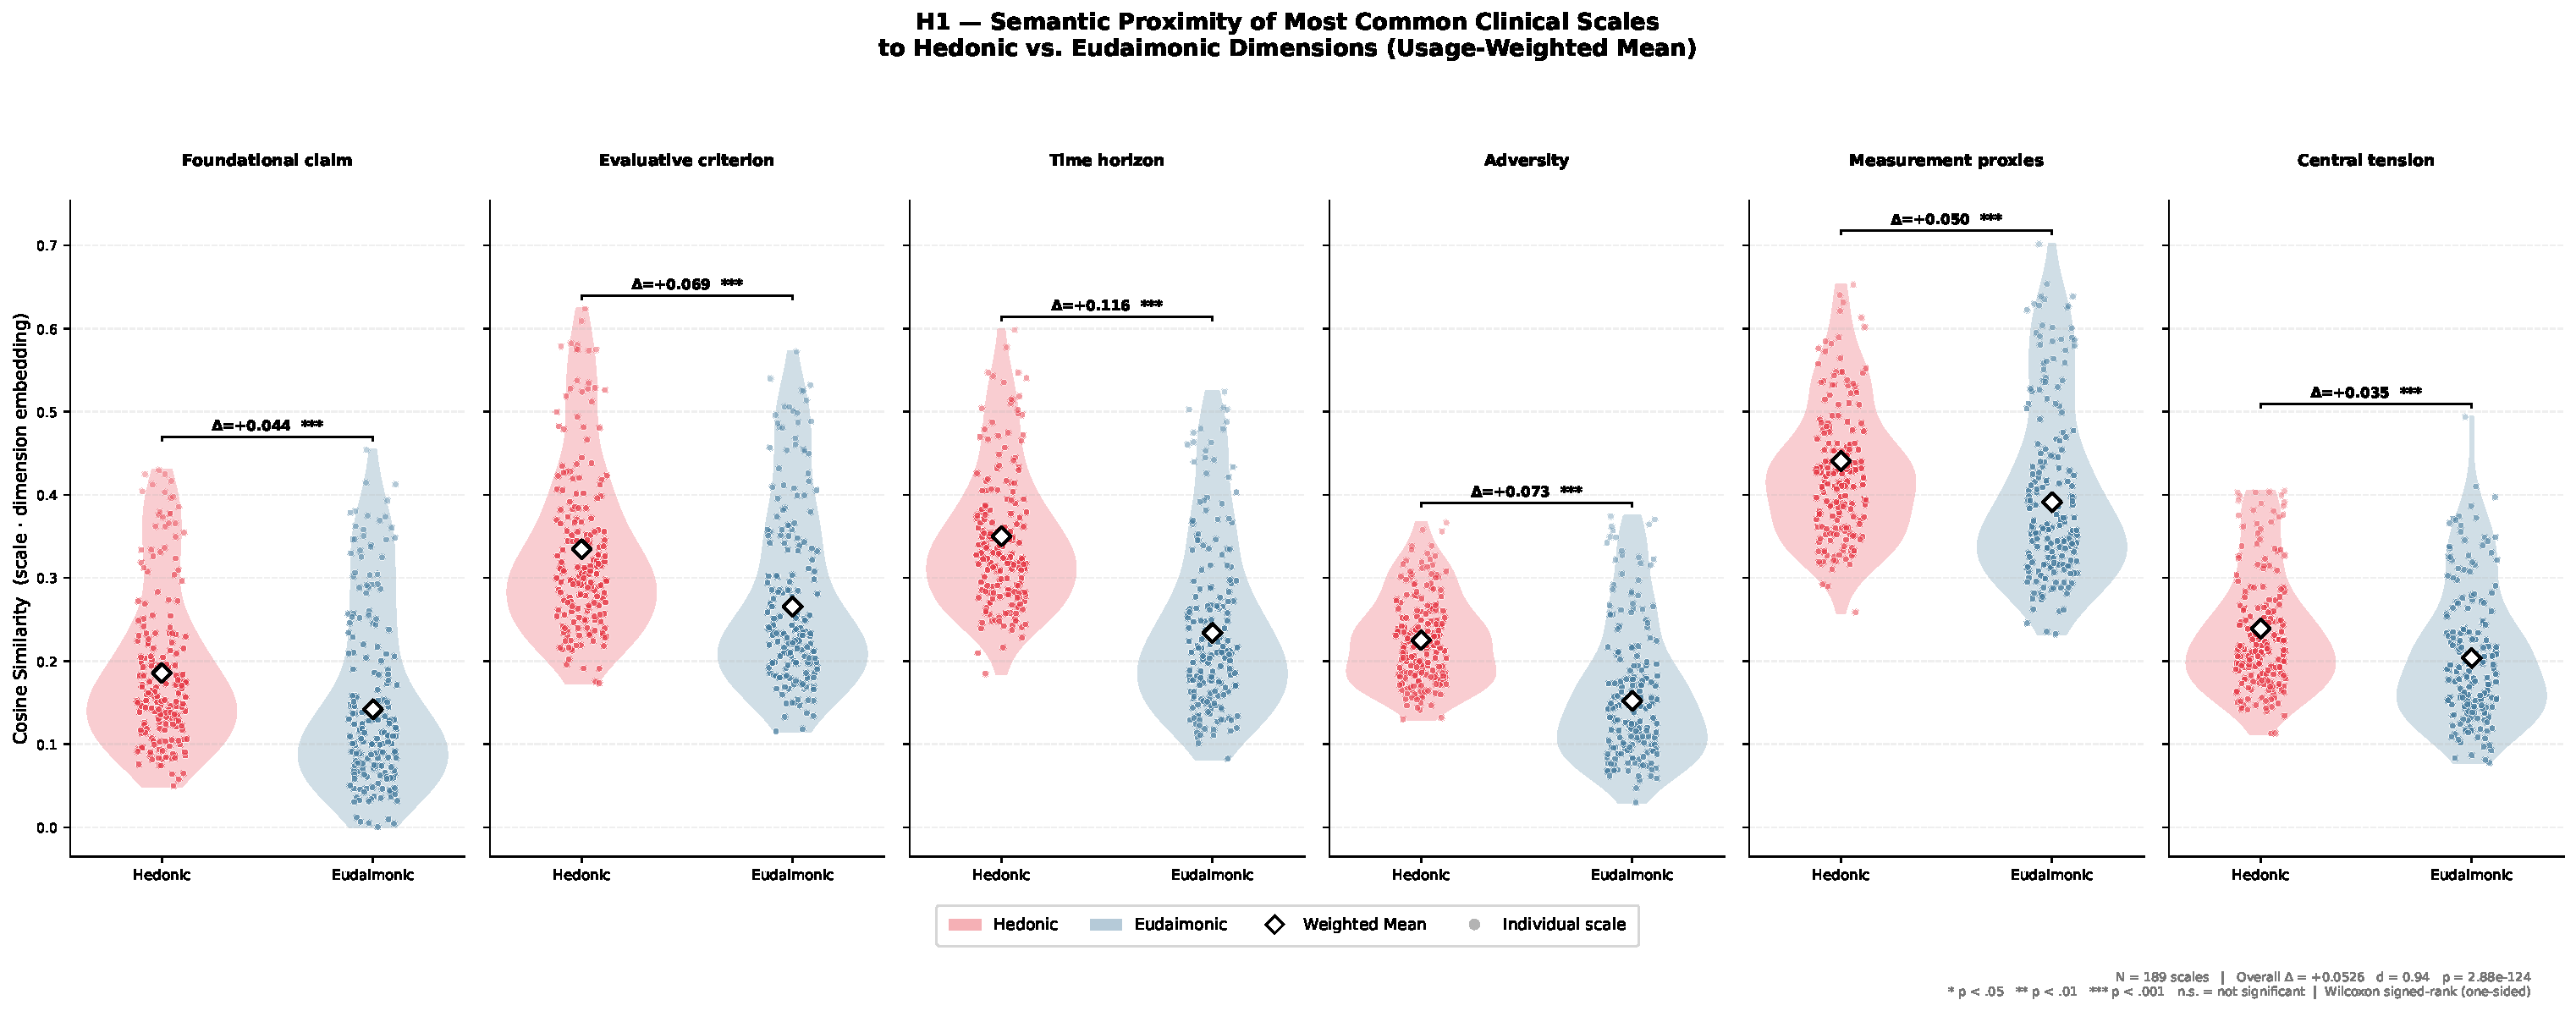
\includegraphics[width=\textwidth]{h1_violin_all_weighted.pdf}
    \label{fig:h1_violin_weighted}
    \floatnote{Distribution of cosine similarities between 189 clinical scales and hedonic (red) versus eudaimonic (blue) well-being poles across six dimensions. Diamonds represent usage-weighted means. All differences significant at $p < .001$ (Holm-corrected). Panels: (A) Foundational claim, (B) Evaluative criterion, (C) Time horizon, (D) Adversity, (E) Measurement proxies, (F) Central tension. Weighted $\Delta = +0.064$, $d = 1.31$.}
\end{figure}

\begin{table}[H]
\caption{Per-dimension hedonic--eudaimonic comparison for all clinical scales}
\label{tab:h1_dims}
\small
\begin{tabular}{lccccccc}
\toprule
\textbf{Dimension} & \textbf{Mean $\Delta$} & \textbf{$d$} & \textbf{$r_{\text{rb}}$} & \textbf{Wt.\ $\Delta$} & \textbf{Wt.\ $d$} & \textbf{$p_{\text{adj}}$} \\
\midrule
Foundational claim        & $+0.037$ & $1.19$ & $.88$ & $+0.044$ & $1.61$ & $< .001$ \\
Evaluative criterion      & $+0.056$ & $1.35$ & $.92$ & $+0.069$ & $1.86$ & $< .001$ \\
Time horizon              & $+0.103$ & $2.05$ & $.99$ & $+0.116$ & $2.60$ & $< .001$ \\
Adversity                 & $+0.065$ & $1.19$ & $.86$ & $+0.073$ & $1.65$ & $< .001$ \\
Measurement proxies       & $+0.025$ & $0.36$ & $.46$ & $+0.050$ & $0.91$ & $< .001$ \\
Central tension           & $+0.029$ & $0.68$ & $.69$ & $+0.035$ & $1.00$ & $< .001$ \\
\midrule
\textbf{Overall}       & $\boldsymbol{+0.053}$ & $\boldsymbol{0.94}$ & $\boldsymbol{.81}$ & $\boldsymbol{+0.064}$ & $\boldsymbol{1.31}$ & $\boldsymbol{< .001}$ \\
\bottomrule
\end{tabular}
\floatnote{$r_{\text{rb}}$ = rank-biserial correlation (non-parametric effect size). Wt.\ = usage-weighted. All $p$-values Holm--Bonferroni corrected across six dimensions.}
\end{table}

The top-50 most-cited scales showed a marginally larger bias ($\Delta = +0.064$, $d = 1.23$), consistent with the hypothesis that the most widely adopted instruments are disproportionately hedonic (see Supplementary Figure~\ref{fig:s_top50} for violin plots of this subset).

As a supplementary convergent-validity check, we applied the same embedding-based analysis to a domain-restricted book corpus: 3{,}883 English-language mental-health books from the Internet Archive, filtered at the \textit{book level} by subject metadata (psychology, psychiatry, psychotherapy, and related fields; see Supplementary Note~\ref{sec:s_ngram_h1} for full method).
Notably, the hedonic bias did \textit{not} replicate in this mental-health literature corpus ($\Delta_w = -0.013$, $d_w = -0.45$, $p = 1.0$; all six dimensions non-significant after Holm--Bonferroni correction), indicating that even vocabulary drawn exclusively from mental-health books does not inherently favour hedonic content (Supplementary Note~\ref{sec:s_ngram_h1}).
This dissociation strengthens the clinical finding: the hedonic bias observed in clinical scales appears to be specific to psychometric instrumentation rather than a general property of evaluative language.

\subsection{H2: The Hedonic Bias Is Increasing Over Time}\label{sec:results-h2}

Temporal analysis of usage-weighted $\Delta$ from 2000 to 2025 revealed a statistically significant positive trend for the aggregate series (slope $= +4.59e-04$/year, $R^2 = .940$, $p < .0001$; Figure~\ref{fig:h2_combined}, panel~A).
The high $R^2$ should be interpreted with caution: it reflects the extreme smoothness of publication-frequency time series rather than substantive explanatory power, and low Durbin--Watson statistics (DW $= 0.28$--$0.94$) indicate substantial autocorrelation, inflating the apparent fit.
At the individual dimension level, all six slopes were positive (Table~\ref{tab:h2_trends}): all dimension slopes were positive, suggesting a uniform temporal increase.
The Mann-Kendall test, which is robust to autocorrelation, independently confirmed the monotonic nature of the trend ($S = 297$, $p < .0001$).

Critically, the absolute magnitude of the temporal shift is modest: the aggregate usage-weighted $\Delta$ increased by approximately $+0.011$ units over 25 years---a small fraction of the cross-sectional bias itself ($\Delta = +0.064$).
This suggests that while the hedonic convergence is real and statistically robust, the field is drifting slowly rather than accelerating sharply.
The practical significance of this incremental shift warrants careful interpretation: even small annual changes in the composition of the measurement ecosystem can compound meaningfully over decades, but the absolute change is far smaller than the baseline cross-sectional bias ($\Delta = +0.053$, $d = 0.94$).
Because each scale's embedding is fixed, the temporal variation in $\Delta$ is driven entirely by differential adoption rates---i.e., which scales grow in publication frequency---rather than changes in scale content.
Panel~B of Figure~\ref{fig:h2_combined} presents the baseline-corrected version, anchoring each dimension at zero in 2000.
A supplementary temporal analysis of 3{,}883 mental-health books from the Internet Archive over 120~years (1900--2019) revealed that the hedonic loading of mental-health literature has been increasing over time (aggregate slope $= +1.09 \times 10^{-5}$/yr, $R^2 = .21$, $p < 10^{-7}$; Mann-Kendall $S = 2{,}152$, $p < 10^{-6}$), paralleling the 25-year clinical trend but with a 42-fold smaller effect size---consistent with the interpretation that hedonic bias is concentrated in psychometric instrumentation rather than broad mental-health discourse (Supplementary Note~\ref{sec:s_ngram_h2}).

\begin{figure}[H]
    \centering
    \caption{Temporal evolution of hedonic measurement bias per dimension, 2000--2025}
    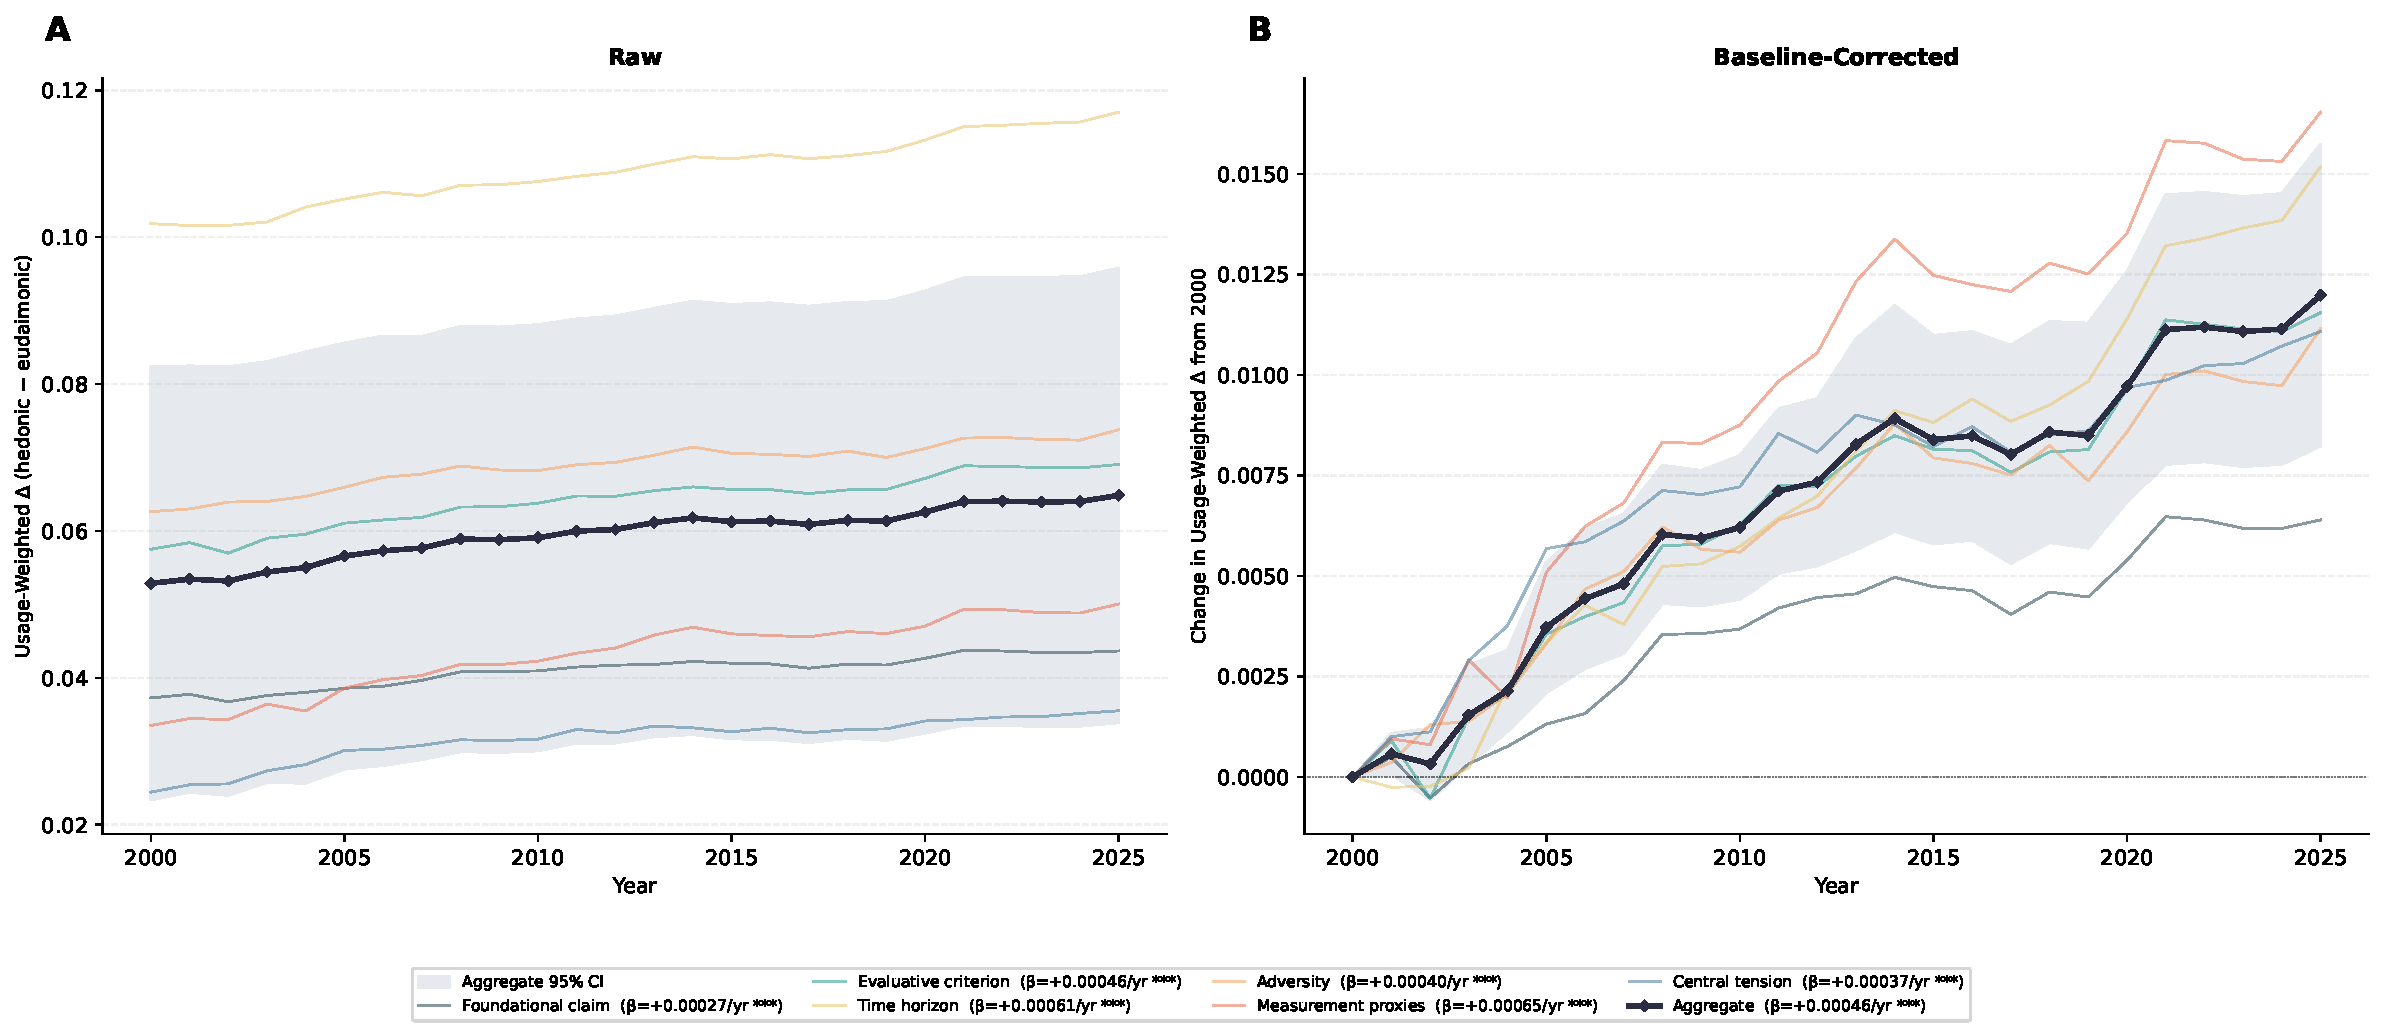
\includegraphics[width=\textwidth]{h2_combined.pdf}
    \label{fig:h2_combined}
    \floatnote{(A) Usage-weighted $\Delta$ (hedonic $-$ eudaimonic) for each dimension and the aggregate, 2000--2025. Shaded ribbon = pointwise 95\% CIs from cross-dimension variability. All six dimension slopes positive. (B) Baseline-corrected version, anchoring each series at zero in 2000 to highlight the cumulative drift. Because each scale's embedding is fixed, all temporal variation reflects differential adoption rates.}
\end{figure}

\begin{table}[H]
\caption{Per-dimension temporal trend statistics, 2000--2025}
\label{tab:h2_trends}
\small
\begin{tabular}{lcccccc}
\toprule
\textbf{Dimension} & \textbf{Slope ($\times 10^{-4}$/yr)} & \textbf{$R^2$} & \textbf{$p_{\text{OLS}}$} & \textbf{MK $S$} & \textbf{MK $p$} & \textbf{DW} \\
\midrule
Foundational claim        & $+2.69$ & $.898$ & $< .001$ & $271$ & $< .001$ & $0.53$ \\
Evaluative criterion      & $+4.60$ & $.932$ & $< .001$ & $283$ & $< .001$ & $0.65$ \\
Time horizon              & $+6.05$ & $.977$ & $< .001$ & $311$ & $< .001$ & $0.94$ \\
Adversity                 & $+4.00$ & $.910$ & $< .001$ & $279$ & $< .001$ & $0.54$ \\
Measurement proxies       & $+6.48$ & $.931$ & $< .001$ & $285$ & $< .001$ & $0.54$ \\
Central tension           & $+3.70$ & $.842$ & $< .001$ & $285$ & $< .001$ & $0.28$ \\
\midrule
\textbf{Aggregate}   & $\boldsymbol{+4.59}$ & $\boldsymbol{.940}$ & $\boldsymbol{< .001}$ & $\boldsymbol{297}$ & $\boldsymbol{< .001}$ & $\boldsymbol{0.43}$ \\
\bottomrule
\end{tabular}
\floatnote{OLS = ordinary least squares; MK = Mann-Kendall; DW = Durbin--Watson. All $p$-values Holm--Bonferroni corrected.}
\end{table}

The Durbin--Watson statistics (DW $= 0.28$--$0.94$) indicate substantial positive autocorrelation in the residuals, which is expected given the smooth, slowly evolving nature of publication patterns.
The converging evidence from both OLS and the non-parametric Mann-Kendall test---which makes no distributional assumptions---provides robust confirmation of the temporal trend.

\subsection{Post-Hoc and Robustness Analyses}\label{sec:results-posthoc}

\subsubsection{Permutation Test}

The observed mean $\Delta = +0.053$ fell in the right tail of the permutation null distribution (null mean $= +0.0002$, null SD $= 0.024$), yielding $p < .0001$ (one-sided; Supplementary Figure~\ref{fig:s_permutation}).
This confirms that the hedonic bias is not an artefact of the dimensional framework: randomly reassigning hedonic and eudaimonic labels produces near-zero average differences.

\subsubsection{Sensitivity to Corpus Size and Usage--Bias Correlation}

The effect size was remarkably stable across corpus sizes: Cohen's $d_{\text{raw}}$ ranged from $1.26$ (top-189) to $1.82$ (top-20), with no evidence of dilution at larger $N$ (Table~\ref{tab:sensitivity}; Figure~\ref{fig:sensitivity_usage}, panel~A).
The usage-weighted mean $\Delta$ converged to approximately $+0.065$ for $N \geq 100$, indicating that the bias is a property of the scale ecosystem rather than a few outlier instruments.
Notably, the raw $\Delta$ decreases monotonically as corpus size grows (from $+0.064$ at $N=20$ to $+0.053$ at $N=189$), while the usage-weighted $\Delta$ remains stable ($\approx +0.065$).
This pattern is explained by the significant positive Spearman correlation between scale usage weight and mean $\Delta$ ($\rho = .226$, $p = .002$; Figure~\ref{fig:sensitivity_usage}, panel~B): more widely adopted scales tend to carry greater hedonic loading, so adding less-used scales dilutes the raw average but not the usage-weighted estimate.

\begin{table}[H]
\caption{Sensitivity analysis of effect size as a function of corpus size}
\label{tab:sensitivity}
\small
\begin{tabular}{rccccc}
\toprule
\textbf{Top-$N$} & \textbf{$\Delta_{\text{raw}}$} & \textbf{$d_{\text{raw}}$} & \textbf{$\Delta_{\text{wt}}$} & \textbf{$d_{\text{wt}}$} \\
\midrule
 20 & $+0.064$ & $1.82$ & $+0.067$ & $2.21$ \\
 50 & $+0.064$ & $1.66$ & $+0.066$ & $1.95$ \\
100 & $+0.060$ & $1.61$ & $+0.065$ & $1.91$ \\
150 & $+0.057$ & $1.48$ & $+0.065$ & $1.88$ \\
189 & $+0.053$ & $1.26$ & $+0.064$ & $1.88$ \\
\bottomrule
\end{tabular}
\floatnote{$\Delta$ = mean hedonic--eudaimonic differential; $d$ = Cohen's $d$; subscript wt = usage-weighted. Both raw and weighted estimates remain stable as corpus size increases, confirming that the bias is a property of the scale ecosystem rather than of a few outlier instruments.}
\end{table}

\begin{figure}[H]
    \centering
    \caption{Sensitivity to corpus size and relationship between scale usage and hedonic loading}
    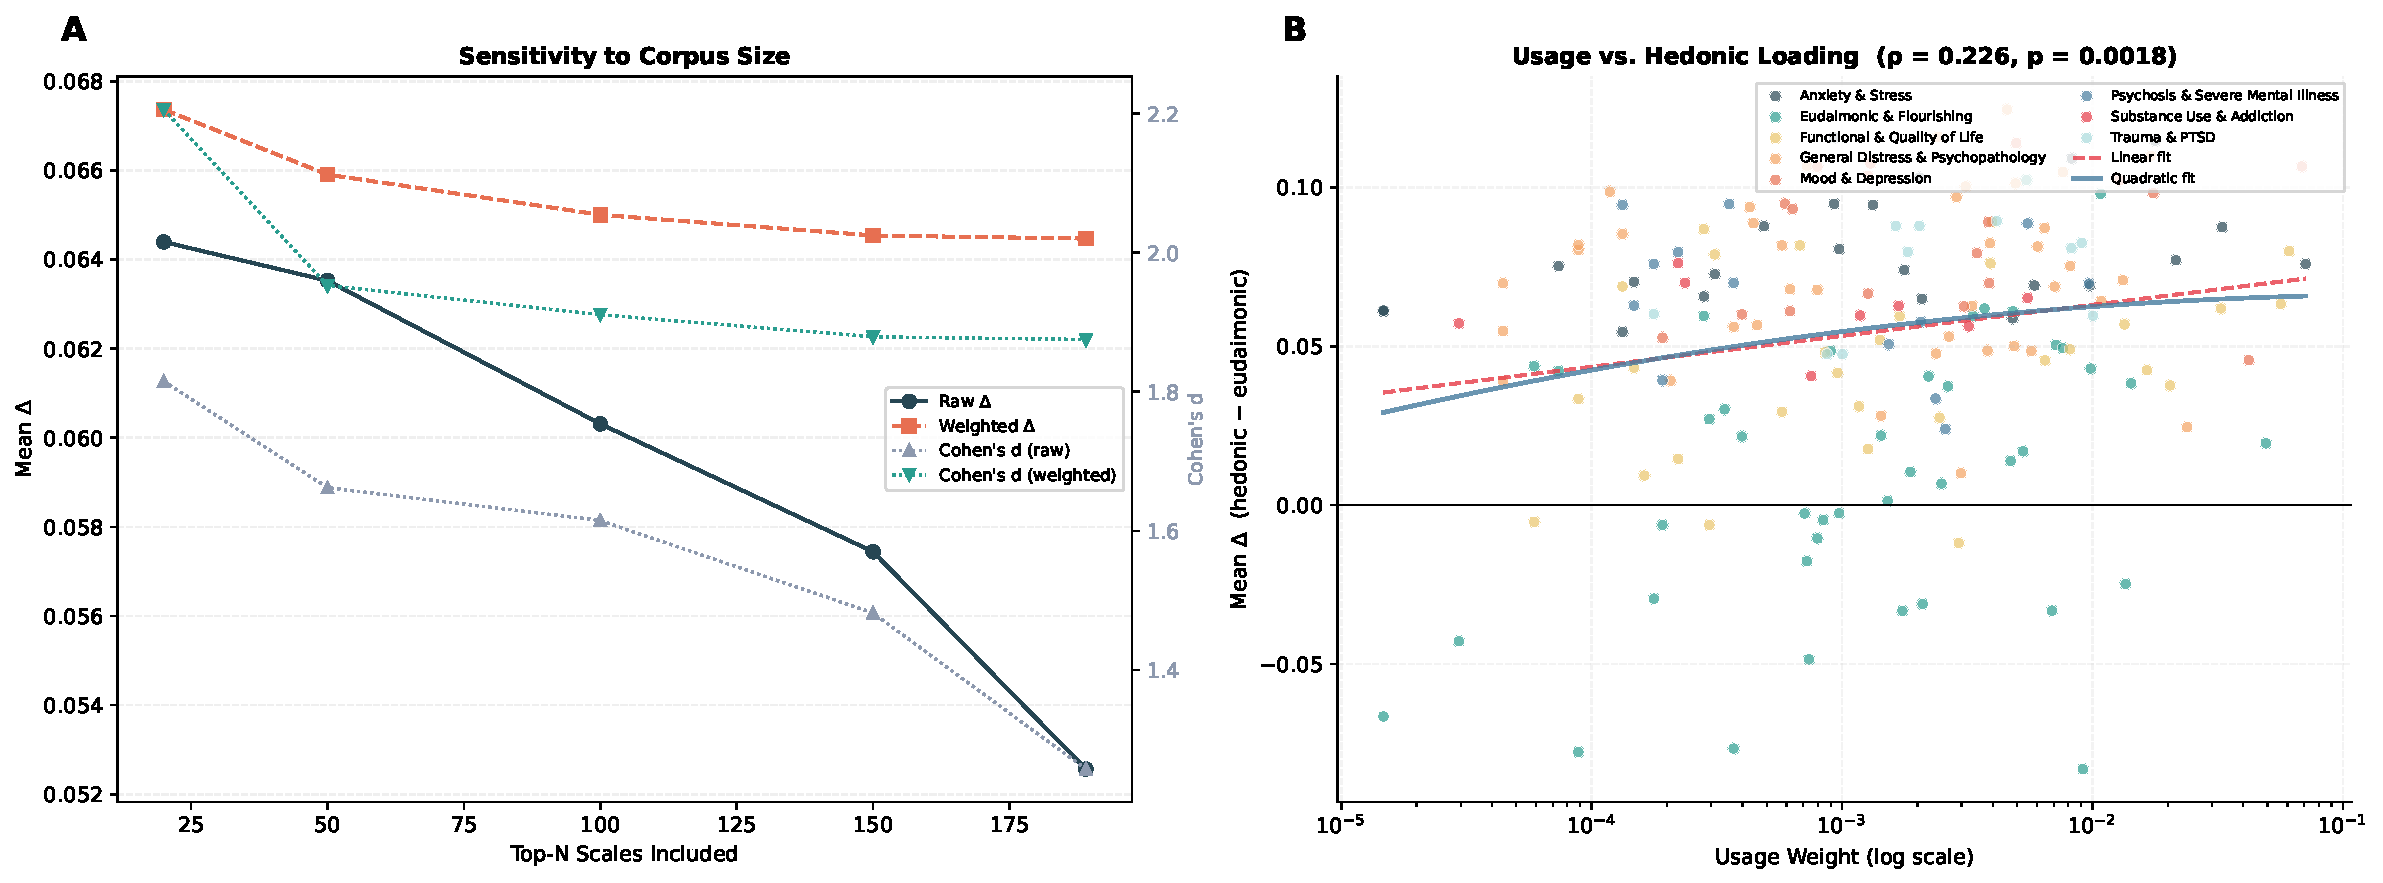
\includegraphics[width=\textwidth]{posthoc_sensitivity_usage_combined.pdf}
    \label{fig:sensitivity_usage}
    \floatnote{(A)~Mean~$\Delta$ (raw and usage-weighted) and Cohen's~$d$ as a function of the number of scales included (top-$N$ by citation count). Raw~$\Delta$ decreases with $N$ while weighted~$\Delta$ remains stable. (B)~Scatter plot of scale-level usage weight vs.\ mean~$\Delta$, coloured by clinical domain. Spearman $\rho = .226$ ($p = .002$). The positive correlation explains the sensitivity pattern: more widely adopted scales carry stronger hedonic loading, so adding less-used scales dilutes the raw average without affecting the usage-weighted estimate.}
\end{figure}

\subsubsection{Domain-Level Analyses}

Seven of eight clinical domains showed a significant cross-sectional hedonic bias after Holm correction (Table~\ref{tab:domain_h1}; Figure~\ref{fig:domain_combined}, panel~A).
The sole exception was Eudaimonic \& Flourishing ($\Delta = +0.008$, $d = 0.18$, $p_{\text{adj}} = .097$), which is expected given that this domain was specifically constructed to include scales targeting eudaimonic constructs.
Notably, even these scales showed a slight (non-significant) hedonic lean, suggesting that the semantic space of clinical measurement is pervasively tilted toward hedonic content.
The strongest hedonic loadings were observed for Substance Use \& Addiction ($d = 5.75$), Anxiety \& Stress ($d = 4.44$), and Trauma \& PTSD ($d = 4.29$).

\begin{table}[H]
\caption{Hedonic bias by clinical domain}
\label{tab:domain_h1}
\small
\begin{tabular}{lcccl}
\toprule
\textbf{Domain} & \textbf{$n$} & \textbf{$\Delta$} & \textbf{$d$} & \textbf{$p_{\text{adj}}$} \\
\midrule
Substance Use \& Addiction                         &  8 & $+0.061$ & $5.75$ & $.008$ \\
Anxiety \& Stress                                  & 23 & $+0.080$ & $4.44$ & $< .001$ \\
Trauma \& PTSD                                     & 10 & $+0.072$ & $4.29$ & $.003$ \\
Mood \& Depression                                 & 18 & $+0.084$ & $3.84$ & $< .001$ \\
Psychosis \& Severe Mental Illness                 & 13 & $+0.065$ & $2.82$ & $< .001$ \\
General Distress \& Psychopathology                & 39 & $+0.072$ & $2.73$ & $< .001$ \\
Functional \& Quality of Life                      & 29 & $+0.045$ & $1.59$ & $< .001$ \\
Eudaimonic \& Flourishing                          & 49 & $+0.008$ & $0.18$ & $.097$ \\
\bottomrule
\end{tabular}
\floatnote{All $p$-values Holm--Bonferroni corrected across eight domains.}
\end{table}

Domain-level temporal trends (Table~\ref{tab:domain_h2}; Figure~\ref{fig:domain_combined}, panel~B) revealed heterogeneous patterns.
Eudaimonic \& Flourishing showed the largest positive slope ($+0.0090$/decade), reflecting the growing but still insufficient adoption of eudaimonic instruments.
Mood \& Depression ($+0.0088$/decade) and Functional \& QoL ($+0.0045$/decade) also showed significant positive trends.
General Distress \& Psychopathology and Psychosis \& SMI showed small but significant negative slopes (total 25-year change $<\!-0.011$), possibly reflecting more nuanced instrumentation.

\begin{table}[H]
\caption{Temporal trends in hedonic bias by clinical domain}
\label{tab:domain_h2}
\small
\begin{tabular}{lccccl}
\toprule
\textbf{Domain} & \textbf{$n$} & \textbf{$\Delta$/decade} & \textbf{Total $\Delta$ (25\,yr)} & \textbf{$R^2$} & \textbf{$p_{\text{adj}}$} \\
\midrule
Eudaimonic \& Flourishing                     & 49 & $+0.0090$ & $+0.022$ & $.769$ & $< .001$ \\
Mood \& Depression                            & 18 & $+0.0088$ & $+0.022$ & $.947$ & $< .001$ \\
Functional \& QoL                             & 29 & $+0.0045$ & $+0.011$ & $.966$ & $< .001$ \\
Substance Use \& Addiction                    &  8 & $+0.0021$ & $+0.005$ & $.833$ & $< .001$ \\
Anxiety \& Stress                             & 23 & $+0.0018$ & $+0.005$ & $.936$ & $< .001$ \\
Trauma \& PTSD                                & 10 & $+0.0009$ & $+0.002$ & $.137$ & $.063$ \\
Gen.\ Distress \& Psychopathology             & 39 & $-0.0026$ & $-0.006$ & $.612$ & $< .001$ \\
Psychosis \& SMI                              & 13 & $-0.0043$ & $-0.011$ & $.831$ & $< .001$ \\
\bottomrule
\end{tabular}
\floatnote{All $p$-values Holm--Bonferroni corrected. $\Delta$/decade = slope per decade; Total $\Delta$ = cumulative change over 25 years.}
\end{table}

\begin{figure}[H]
    \centering
    \caption{Domain-level hedonic bias: cross-sectional magnitude and temporal trends}
    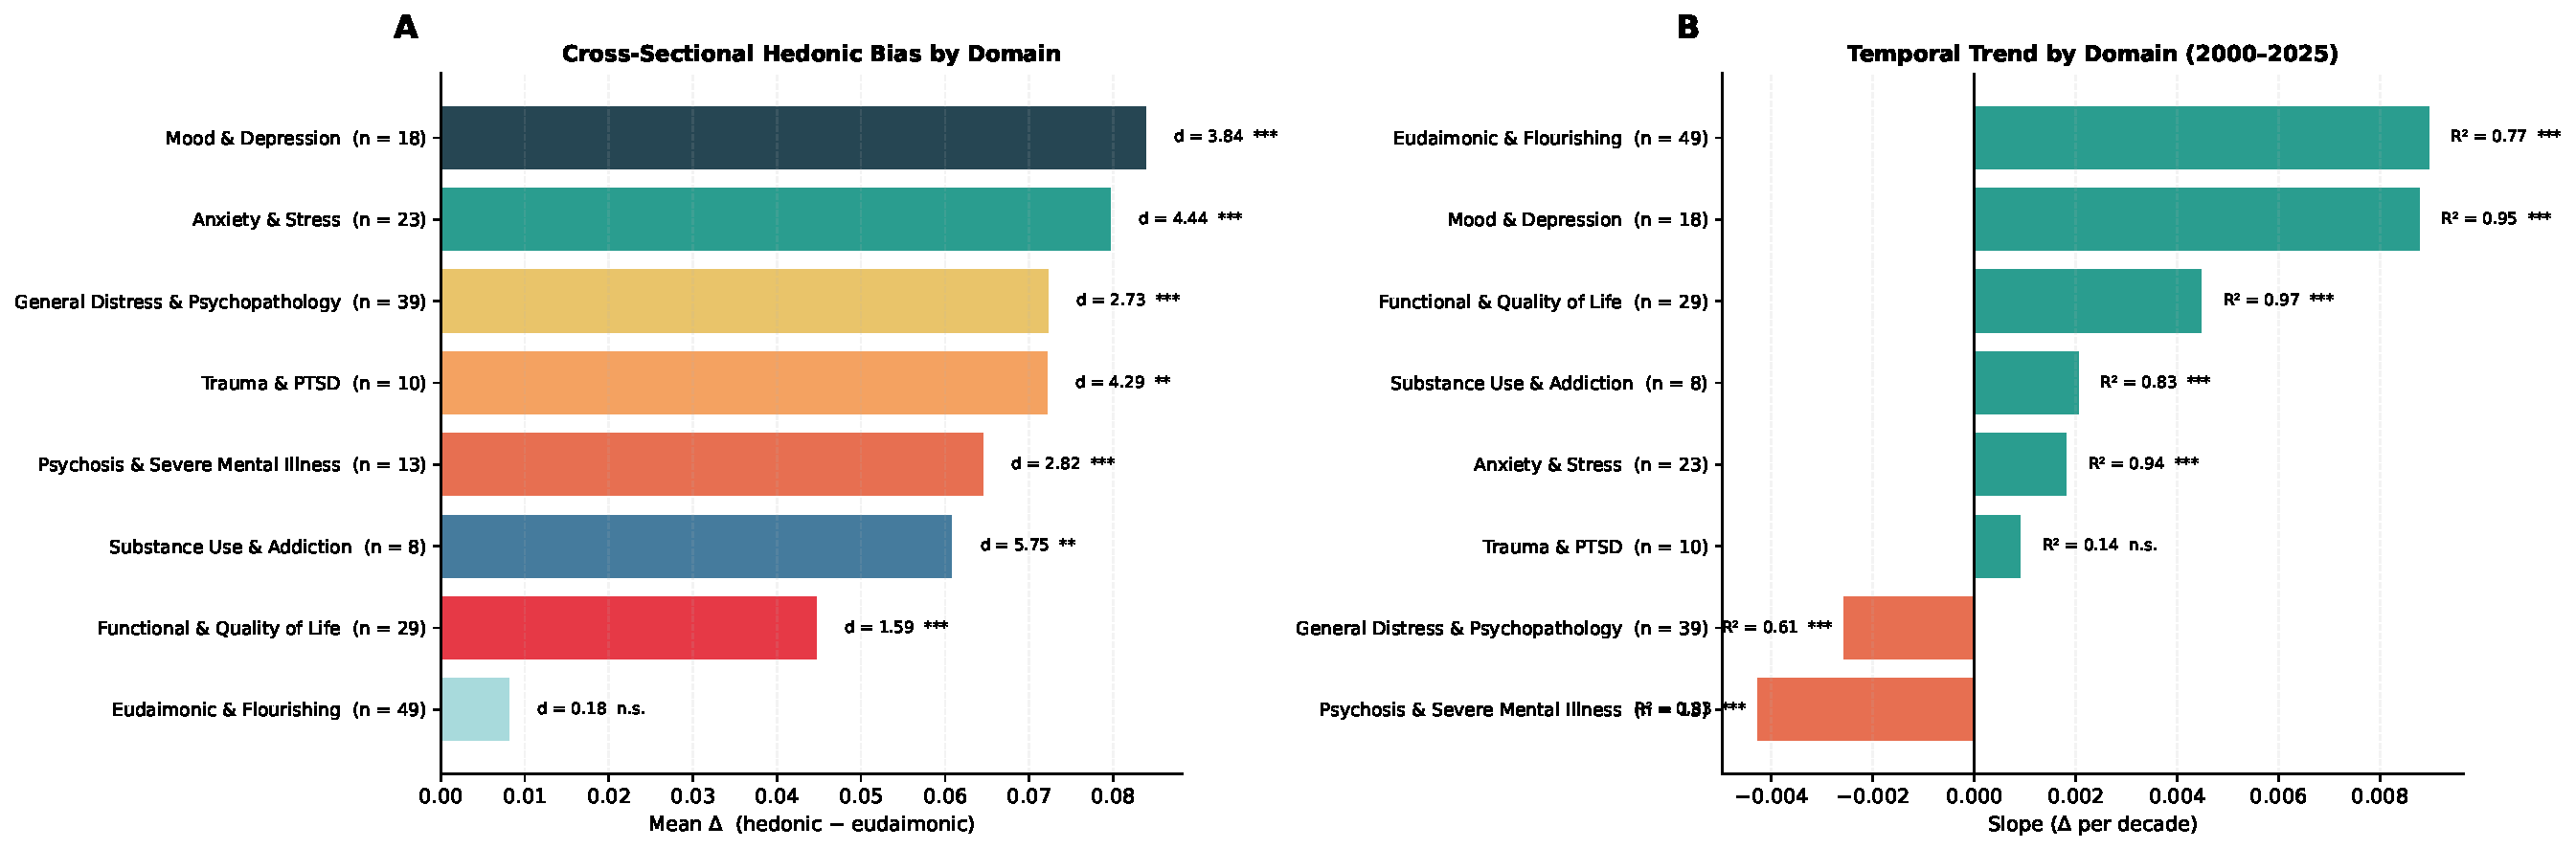
\includegraphics[width=\textwidth]{posthoc_domain_combined.pdf}
    \label{fig:domain_combined}
    \floatnote{(A)~Cross-sectional hedonic bias by clinical domain (mean~$\Delta$) with Cohen's~$d$ and Holm-corrected significance. All domains except Eudaimonic \& Flourishing show significant hedonic loading. (B)~Temporal trend (slope per decade) by domain. Green bars indicate increasing hedonic bias; orange bars indicate decreasing. Most domains show increasing hedonic convergence over 2000--2025.}
\end{figure}

\subsubsection{Post-Hoc: Methodological Utility as a Covariate}

The Time horizon dimension showed the largest cross-sectional effect ($d = 2.05$ raw, $d = 2.60$ weighted), which is consistent with a methodological utility explanation: scales that assess present-moment states (current mood, symptom severity over the past two weeks) are inherently more amenable to short-duration clinical trials and generate more interpretable change scores than instruments probing long-term narrative identity or growth trajectories.
If methodological tractability partly drives scale adoption, we would expect dimensions most closely aligned with RCT-compatible constructs to show the strongest hedonic loading---and this is precisely what we observe.

To test this, we examined whether the six dimensions' effect sizes correlate with a rough ordinal ranking of their ``RCT compatibility'' (Time horizon and Measurement proxies ranked highest; Central tension and Foundational claim ranked lowest, as more abstract constructs).
The rank-order correlation between dimension-level $d$ and RCT compatibility was $r_s = .77$ ($p = .10$, $n = 6$), directionally consistent with the methodological utility hypothesis but not significant given the small number of dimensions.
This suggestive finding motivates future research decomposing the hedonic bias into philosophical versus methodological components.

% ══════════════════════════════════════════════════════════════════════
\section{Discussion}\label{sec:discussion}
% ══════════════════════════════════════════════════════════════════════

\subsection{Summary of Findings}

This study provides the first large-scale, quantitative evidence that the Western mental healthcare assessment ecosystem is systematically biased toward hedonic conceptions of well-being.
Using semantic embeddings of 189 clinical scales, we demonstrated that across all six theoretically derived hedonic--eudaimonic dimensions, clinical scales are significantly and substantially closer to hedonic poles ($d = 0.91$--$2.60$ usage-weighted; all $p_{\text{adj}} < .001$).
This bias is robust to usage-weighting, corpus size, and permutation-based null testing.

The temporal analysis (H2) reveals a statistically significant but modest drift: the usage-weighted hedonic loading has increased by approximately $+0.011$ units over 25 years, driven entirely by differential adoption rates rather than changes in scale content (since each scale's embedding is fixed, all temporal variation in $\Delta$ reflects which scales grow in publication frequency).
The high $R^2$ values should be attributed to the smoothness of publication-frequency time series rather than interpreted as evidence of a powerful temporal effect.
The annual increment ($+0.00046$) is small in absolute terms, but its unidirectional persistence over a quarter-century---confirmed by both parametric and non-parametric tests---points to a structural trajectory in which hedonically oriented instruments are steadily gaining relative prominence.
The pattern is pervasive across clinical domains, with even nominally eudaimonic scales showing a slight (non-significant) hedonic lean.

\subsection{Theoretical Implications}

Our findings converge with longstanding arguments in the well-being literature.
\citet{ryan2001happiness} and \citet{deci2000self} emphasised that hedonic and eudaimonic well-being are conceptually and empirically distinct, yet our data show that the measurement tools available to clinicians overwhelmingly probe only one side of this distinction.
\citet{keyes2002mental} called for a ``complete state model'' of mental health that includes both symptom absence and positive functioning; two decades later, our analysis suggests that clinical measurement has not caught up with this theoretical mandate.
Perhaps most strikingly, the WHO's own definition of mental health---emphasising self-realisation, productive functioning, and community contribution \citep{who2004mental}---is fundamentally eudaimonic, yet the instruments most widely deployed to assess mental health remain overwhelmingly hedonic.

The finding that the Time horizon dimension shows the largest effect ($d = 2.60$) is particularly striking.
Clinical scales predominantly assess present-moment states---current mood, recent symptom severity, functional status over the past two weeks---while eudaimonic conceptions emphasise long-term trajectories of growth, narrative identity, and purpose development
\citep{mcadams2001psychology, king2004benefit}.
This temporal myopia may cause clinicians and researchers to miss meaningful recovery that unfolds over months or years
\citep{tedeschi2004posttraumatic}.

\subsection{Practical Implications}

The hedonic predominance documented in H1 and the modest but persistent temporal drift documented in H2 have direct consequences for clinical practice and health policy in Western mental healthcare.

\subsubsection{Treatment Evaluation}

If primary outcomes are defined in hedonic terms---symptom reduction, mood improvement, subjective distress---then interventions targeting meaning, autonomy, or personal growth may appear ineffective even when they produce substantial eudaimonic gains \citep{seligman2005positive, sin2009enhancing, wong2011what}.
This asymmetry is not merely academic: regulatory approval, insurance reimbursement, and clinical guideline inclusion all depend on demonstrating efficacy through validated outcome measures.
When those measures are overwhelmingly hedonic, the evidentiary base is structurally tilted against eudaimonic interventions regardless of their actual effectiveness.

\subsubsection{Resource Allocation}

Funding bodies and regulatory agencies that rely on standardised outcomes (e.g., NICE, FDA) may systematically undervalue eudaimonic interventions, creating a self-reinforcing cycle in which hedonic instruments receive more validation studies, further entrenching their dominance \citep{vittersø2016handbook}.
Grant review panels, trained to evaluate proposals against established outcome measures, may inadvertently penalise research that employs newer eudaimonic instruments with shorter psychometric track records.

\subsubsection{Patient Perspectives}

Qualitative research consistently indicates that patients value meaning, purpose, and personal growth alongside---and sometimes above---symptom relief \citep{slade2010mental, davidson2008recovery}.
The recovery movement in mental health has long emphasised that ``getting better'' encompasses far more than symptom reduction, yet the current measurement infrastructure cannot fully capture these priorities.
The gap between what patients report as meaningful recovery and what clinicians can measure with standard instruments represents a significant validity threat to patient-centred care.

\subsubsection{Assessment Design}

Our findings provide an empirical foundation for developing next-generation assessment tools that balance hedonic and eudaimonic content.
The dimensional framework (Table~\ref{tab:dimensions}) could guide systematic item generation to ensure balanced coverage of both traditions.
Crucially, this does not require abandoning existing hedonic instruments but rather supplementing them with validated eudaimonic measures to achieve the ``complete state'' model of mental health that \citet{keyes2002mental} envisioned.

\subsection{The Methodological Utility Hypothesis}

An important alternative---or complementary---explanation for the observed hedonic predominance and its temporal intensification concerns the differential \textit{methodological utility} of hedonic versus eudaimonic constructs.
Hedonic states such as depressed mood, anxiety severity, and subjective distress are, by their nature, more amenable to the biomedical framework that dominates Western clinical research.
Symptom frequency counts, Likert-scaled affect ratings, and somatic complaint inventories yield interval-like data that map naturally onto randomised controlled trial (RCT) designs, dose--response curves, and regulatory endpoints.
Eudaimonic constructs---meaning, purpose, personal growth, virtue---resist such neat quantification.
They are inherently contextual, temporally extended, and difficult to operationalise as discrete outcome variables within a two-week assessment window.

This asymmetry creates a structural selection pressure at the level of scale development.
Instruments that produce clean, reliable change scores in short-duration trials are more likely to be adopted as primary outcomes, validated in multiple populations, and cited in subsequent studies---all of which inflate their PubMed presence.
The observed temporal trend (H2) may therefore reflect not only a deepening philosophical commitment to hedonic conceptions but also the growing dominance of RCT methodology in evidence-based medicine, which rewards precisely the kind of measurement that hedonic scales provide.
In other words, the hedonic bias may be partly an artefact of the measurement infrastructure's optimisation for statistical tractability rather than conceptual completeness.

The supplementary book-corpus analysis (Supplementary Notes~\ref{sec:s_ngram_h1}--\ref{sec:s_ngram_h2}) provides converging evidence for this interpretation.
Mental-health literature---textbooks, monographs, and research volumes---does \textit{not} exhibit a cross-sectional hedonic bias ($\Delta_w = -0.013$, $p = 1.0$), yet its hedonic loading has been increasing significantly over 120~years (slope $= +1.09 \times 10^{-5}$/yr, $R^2 = .21$, $p < 10^{-7}$).
Critically, the temporal effect in books is approximately 42~times smaller than the corresponding clinical-scale trend, demonstrating that the hedonic bias is dramatically concentrated in psychometric instruments.
This pattern is consistent with the methodological-utility account: the broader disciplinary discourse engages extensively with eudaimonic constructs, but this conceptual breadth is progressively filtered out when vocabulary is funnelled through the narrow aperture of instrument design, where hedonic items offer greater psychometric tractability---higher test--retest reliability, cleaner factor loadings, and more straightforward sensitivity to change in short-duration trials.

This interpretation does not diminish the practical significance of the bias.
Whether the cause is philosophical preference, methodological convenience, or institutional inertia, the consequence is the same: the assessment ecosystem systematically under-represents eudaimonic well-being, and this under-representation may subtly shape societal conceptions of mental health by privileging symptom-focused evaluative frameworks in public discourse, policy, and self-understanding.
Recognising the role of methodological utility suggests that addressing the imbalance will require not only new instruments but also new trial designs---longitudinal, mixed-methods, and qualitatively enriched---that can accommodate the temporal and contextual complexity of eudaimonic constructs.

\subsection{Beyond Embeddings: Patient-Level Validation}

While semantic embeddings provide a scalable and objective method for quantifying the hedonic--eudaimonic balance at the instrument level, a complementary---and arguably more direct---approach would involve analysing large-scale patient-level response data.
If clinical datasets containing responses to both hedonic and eudaimonic instruments were available, principal component analysis (PCA) of the combined item correlation matrix could reveal whether the latent variance structure mirrors the embedding-based findings.
Specifically, one could test whether the principal components that explain the most patient-reported variance load disproportionately onto items with hedonic content, and whether the hedonic--eudaimonic loading differential on these components increases across successive measurement cohorts.
Such an analysis would provide convergent validity from actual patient conceptualisations of their own well-being, rather than from the semantic content of assessment tools alone.
The present embedding-based methodology establishes the structural bias; patient-level PCA would confirm whether this structural bias translates into a corresponding asymmetry in the variance captured by routine clinical assessment.

\subsection{Methodological Considerations}

The use of semantic embeddings as a measurement tool introduces both strengths and limitations.
On the strength side, embeddings provide a continuous, high-dimensional measure of semantic content that avoids binary categorisation.
The \texttt{text-embedding-3-large} model was trained on a diverse web corpus, capturing nuanced semantic relationships that keyword-based approaches would miss.

However, several methodological considerations warrant discussion.
First, embeddings reflect the distributional semantics of training data \citep{bender2021dangers}.
If the training corpus itself over-represents hedonic language in clinical contexts, the embeddings may amplify existing biases rather than providing a neutral measurement.
We mitigated this concern through the permutation test, which confirmed that the observed bias exceeds what would be expected under random labelling.

Second, the choice of six dimensions, while theoretically grounded, is necessarily selective.
Alternative dimensional frameworks might yield different effect sizes, though we expect the direction of the bias would be preserved given its consistency across all six dimensions tested.

Third, PubMed publication counts are an imperfect proxy for clinical usage.
Scales may be widely used in practice without generating proportional academic citations, and publication trends reflect research priorities rather than clinical deployment.

\subsection{Durbin--Watson, Autocorrelation, and the Paradox of High $R^2$}

The low Durbin--Watson statistics (DW $= 0.28$--$0.94$) indicate positive autocorrelation in the H2 residuals, which is expected for slowly evolving time series.
While this inflates the precision of OLS standard errors, three factors mitigate concern: (a) the Mann-Kendall test, which is non-parametric and robust to autocorrelation, independently confirms all trends; (b) bootstrap confidence intervals on slopes do not assume independence; and (c) for most dimensions, the high $R^2$ values indicate that the linear trend captures the dominant signal, leaving little residual structure to exploit.

However, the high $R^2$ values observed for several dimensions warrant critical scrutiny.
Usage-weighted time series of publication frequencies are inherently smooth: year-to-year fluctuations in which scales are cited are small relative to the long-term structural composition of the literature.
Any monotonically increasing quantity regressed against time will yield a high $R^2$ if the noise is sufficiently small relative to the trend.
Consequently, the $R^2$ here primarily reflects the smoothness of the data rather than the substantive strength of the temporal effect.
The more informative statistic is the absolute slope: $+4.6 \times 10^{-4}$/year amounts to $+0.011$ over 25 years---a real but modest shift relative to the cross-sectional effect size ($\Delta = +0.053$, $d = 0.94$).

\subsection{Magnitude of the Temporal Shift}

The distinction between statistical significance and practical significance is crucial for interpreting H2.
The temporal trend is statistically unambiguous ($p < .001$ by multiple tests), but the absolute annual increment ($+0.00046$ per year) is extremely small.
In context, 25 years of publication shifts have produced a change in the effective hedonic loading equivalent to only a small fraction of the static bias.
Whether this incremental drift carries meaningful consequences for clinical practice depends on one's perspective: on one hand, the cross-sectional predominance (H1) is by far the larger concern; on the other, even slow unidirectional drift in a measurement ecosystem compounds over decades and reflects a structural trajectory that, if continued, would further entrench hedonic dominance.

% ══════════════════════════════════════════════════════════════════════
\section{Limitations}\label{sec:limitations}
% ══════════════════════════════════════════════════════════════════════

\subsection{Embedding Model Dependence}

Our results rely on a single embedding model (OpenAI's \texttt{text-embedding-3-large}).
Although this model demonstrates strong performance on semantic similarity benchmarks and the large, consistent effect sizes observed here suggest robustness, replication with alternative architectures---such as sentence-BERT \citep{devlin2019bert}, Cohere Embed, or open-source models like E5 or GTE---would strengthen confidence in the generality of these findings.
The distributional semantics learned by any model reflect properties of its training corpus \citep{bender2021dangers}, and systematic differences in corpus composition across models could shift effect sizes.

\subsection{Scale Representation}

Scales were represented by brief textual descriptions (full name, abbreviation, and a one-sentence construct summary) rather than complete item content.
This approach captures construct-level semantics efficiently but necessarily loses item-level nuance.
Some scales contain individual items that probe eudaimonic constructs even when the overall instrument is classified as hedonic (e.g., several PHQ-9 items address functional impairment rather than pure mood state).
Item-level embedding analysis would provide a more granular view of the hedonic--eudaimonic spectrum within individual instruments.

\subsection{Dimensional Framework}

The six hedonic--eudaimonic dimension pairs were specified \textit{a priori} on the basis of theoretical literature.
While this ensures conceptual grounding, the framework is necessarily selective: alternative dimensional decompositions might yield different effect sizes.
We note, however, that the consistency of the bias across all six dimensions (all $p_{\text{adj}} < .001$) suggests that the finding is not an artefact of any single dimension choice.
Data-driven approaches such as factor analysis of the full scale--pole similarity matrix could complement this theory-driven framework in future work.

\subsection{Operationalisation of Usage}

PubMed publication counts serve as our primary proxy for scale adoption, but this operationalisation has several known limitations that warrant careful consideration.
First, publication counts reflect research usage rather than clinical deployment: a scale may be widely used in routine practice (e.g., the PHQ-9 in primary care screening) without generating proportional academic citations, while a scale with many methodological publications may see limited clinical uptake.
Second, our search queries used standardised abbreviations and full names, but scales that share abbreviations with unrelated terms may yield inflated counts, and scales known primarily by informal names may be under-counted.
Third, PubMed indexes only a subset of the global scientific literature, with known biases toward English-language, biomedical, and Western-institution journals---precisely the domain in which hedonic instruments are most entrenched.
Fourth, multi-instrument studies (e.g., a single trial administering both the PHQ-9 and the WHOQOL-BREF) assign equal credit to each scale, potentially inflating the usage of co-administered instruments.

Alternative operationalisations that could address these limitations include: clinician surveys documenting actual instrument selection in routine practice; electronic health record (EHR) audit data counting scale administrations; analysis of clinical trial registries (e.g., ClinicalTrials.gov) to determine which instruments are specified as primary versus secondary outcomes; and insurance billing code analyses reflecting reimbursed assessments.
Each of these approaches would provide a more direct measure of clinical adoption, though each also introduces its own biases and access constraints.
The convergence of results across multiple operationalisations would substantially strengthen the claim.

\subsection{Language and Cultural Scope}

All analyses were conducted in English using scales developed primarily within Western (North American and European) research traditions.
The hedonic--eudaimonic balance in clinical measurement may differ substantially across languages and cultural contexts.
Non-Western healing traditions---such as Buddhist-informed approaches emphasising equanimity and compassion, or Indigenous frameworks centring community interconnection---may operationalise well-being in ways that transcend the hedonic--eudaimonic dichotomy entirely.
Cross-cultural replication is essential before generalising these findings beyond Western mental healthcare systems.

\subsection{Causal Interpretation}

The temporal trend documented in H2 is observational and correlational; it cannot establish that any single factor \textit{causes} the increasing hedonic bias.
Plausible drivers include shifts in research funding priorities, the growing influence of evidence-based medicine frameworks that favour short-term RCT designs, changes in diagnostic classification systems (e.g., DSM-5 revisions), pharmaceutical industry incentives favouring symptom-reduction endpoints, and evolving population health needs.
Distinguishing among these candidate causes would require quasi-experimental or natural-experiment designs that exploit exogenous shocks to the measurement ecosystem (e.g., the introduction of new clinical guidelines mandating eudaimonic outcomes).
A particularly promising avenue for future work would be to test the methodological-utility pathway causally using structural equation modelling (SEM): for instance, modelling whether instrument psychometric properties (e.g., internal consistency, sensitivity to change, factor simplicity) mediate the relationship between hedonic content and adoption rate, while controlling for publication year, clinical domain, and regulatory context.
Such an approach could disentangle whether hedonic instruments are adopted \textit{because} they are psychometrically convenient or \textit{despite} equivalent psychometric performance of eudaimonic alternatives.

% ══════════════════════════════════════════════════════════════════════
\section{Conclusion}\label{sec:conclusion}
% ══════════════════════════════════════════════════════════════════════

This study provides robust, large-scale evidence that the Western mental healthcare assessment ecosystem systematically privileges hedonic over eudaimonic conceptions of well-being.
The bias is large (Cohen's $d = 0.94$, large effect), pervasive (present across all six dimensions and nearly all clinical domains), temporally increasing, and robust to multiple analytic strategies.
In short, the field's measurement infrastructure is converging toward hedonic optimisation.

These findings do not imply that hedonic measurement is unimportant---symptom relief and positive affect are genuine components of well-being.
Rather, they reveal a structural asymmetry between the WHO's eudaimonic definition of mental health and the hedonic instruments used to measure it.
This asymmetry may reflect not only philosophical preference but also the differential methodological utility of hedonic constructs within dominant research paradigms.

Addressing this convergence will require concerted effort across multiple levels: developing and validating new eudaimonic instruments, incorporating eudaimonic outcomes into clinical trial protocols, designing longitudinal and mixed-methods studies capable of capturing meaning and growth, and updating clinical guidelines to reflect the dual-continuum model of mental health.
The dimensional framework presented here offers a starting point for ensuring that future assessment tools provide balanced coverage of both hedonic and eudaimonic well-being.

% ══════════════════════════════════════════════════════════════════════
% References
% ══════════════════════════════════════════════════════════════════════
\newpage
\bibliographystyle{apalike}

\begin{thebibliography}{99}

\bibitem[Aristotle, 1999]{aristotle1999nicomachean}
Aristotle (1999).
\textit{Nicomachean Ethics} (T. Irwin, Trans., 2nd ed.).
Hackett Publishing.

\bibitem[Bender et~al., 2021]{bender2021dangers}
Bender, E.~M., Gebru, T., McMillan-Major, A., \& Shmitchell, S. (2021).
On the dangers of stochastic parrots: Can language models be too big?
\textit{Proceedings of FAccT '21}, 610--623.
\texttt{doi:10.1145/3442188.3445922}

\bibitem[Bhatia, 2019]{bhatia2019predicting}
Bhatia, S. (2019).
Predicting risk perception: New clues from data science.
\textit{Management Science, 65}(8), 3800--3823.
\texttt{doi:10.1287/mnsc.2018.3121}

\bibitem[Bornmann \& Mutz, 2015]{bornmann2015growth}
Bornmann, L., \& Mutz, R. (2015).
Growth rates of modern science: A bibliometric analysis based on the number of publications and cited references.
\textit{Journal of the Association for Information Science and Technology, 66}(11), 2215--2222.
\texttt{doi:10.1002/asi.23329}

\bibitem[Brown et~al., 2020]{brown2020language}
Brown, T.~B., Mann, B., Ryder, N., et~al. (2020).
Language models are few-shot learners.
\textit{Advances in Neural Information Processing Systems, 33}, 1877--1901.

\bibitem[Caliskan et~al., 2017]{caliskan2017semantics}
Caliskan, A., Bryson, J.~J., \& Narayanan, A. (2017).
Semantics derived automatically from language corpora contain human-like biases.
\textit{Science, 356}(6334), 183--186.
\texttt{doi:10.1126/science.aal4230}

\bibitem[Davidson et~al., 2008]{davidson2008recovery}
Davidson, L., Borg, M., Marin, I., Topor, A., Mezzina, R., \& Sells, D. (2008).
Processes of recovery in serious mental illness: Findings from a multinational study.
\textit{American Journal of Psychiatric Rehabilitation, 8}(3), 177--201.
\texttt{doi:10.1080/15487760500339360}

\bibitem[Deci \& Ryan, 2000]{deci2000self}
Deci, E.~L., \& Ryan, R.~M. (2000).
The ``what'' and ``why'' of goal pursuits: Human needs and the self-determination of behavior.
\textit{Psychological Inquiry, 11}(4), 227--268.
\texttt{doi:10.1207/S15327965PLI1104\_01}

\bibitem[Devlin et~al., 2019]{devlin2019bert}
Devlin, J., Chang, M.-W., Lee, K., \& Toutanova, K. (2019).
BERT: Pre-training of deep bidirectional transformers for language understanding.
\textit{Proceedings of NAACL-HLT}, 4171--4186.
\texttt{doi:10.18653/v1/N19-1423}

\bibitem[Diener, 1984]{diener1984subjective}
Diener, E. (1984).
Subjective well-being.
\textit{Psychological Bulletin, 95}(3), 542--575.
\texttt{doi:10.1037/0033-2909.95.3.542}

\bibitem[Diener et~al., 1985]{diener1985satisfaction}
Diener, E., Emmons, R.~A., Larsen, R.~J., \& Griffin, S. (1985).
The Satisfaction With Life Scale.
\textit{Journal of Personality Assessment, 49}(1), 71--75.
\texttt{doi:10.1207/s15327752jpa4901\_13}

\bibitem[Disabato et~al., 2016]{disabato2016different}
Disabato, D.~J., Goodman, F.~R., Kashdan, T.~B., Short, J.~L., \& Jarden, A. (2016).
Different types of well-being? A cross-cultural examination of hedonic and eudaimonic well-being.
\textit{Psychological Assessment, 28}(5), 471--482.
\texttt{doi:10.1037/pas0000209}

\bibitem[Grand et~al., 2022]{grand2022semantic}
Grand, G., Blank, I.~A., Pereira, F., \& Fedorenko, E. (2022).
Semantic projection recovers rich human knowledge of multiple object features from word embeddings.
\textit{Nature Human Behaviour, 6}(7), 975--987.
\texttt{doi:10.1038/s41562-022-01316-8}

\bibitem[Holm, 1979]{holm1979simple}
Holm, S. (1979).
A simple sequentially rejective multiple test procedure.
\textit{Scandinavian Journal of Statistics, 6}(2), 65--70.

\bibitem[Huppert \& So, 2013]{huppert2009exploring}
Huppert, F.~A., \& So, T.~T.~C. (2013).
Flourishing across Europe: Application of a new conceptual framework for defining well-being.
\textit{Social Indicators Research, 110}(3), 837--861.
\texttt{doi:10.1007/s11205-011-9966-7}

\bibitem[Huta \& Waterman, 2014]{huta2010pursuing}
Huta, V., \& Waterman, A.~S. (2014).
Eudaimonia and its distinction from hedonia: Developing a classification and terminology for understanding conceptual and operational definitions.
\textit{Journal of Happiness Studies, 15}(6), 1425--1456.
\texttt{doi:10.1007/s10902-013-9485-0}

\bibitem[Kahneman et~al., 1999]{kahneman1999hedonic}
Kahneman, D., Diener, E., \& Schwarz, N. (Eds.) (1999).
\textit{Well-being: The Foundations of Hedonic Psychology}.
Russell Sage Foundation.

\bibitem[Kashdan et~al., 2008]{kashdan2008reconsidering}
Kashdan, T.~B., Biswas-Diener, R., \& King, L.~A. (2008).
Reconsidering happiness: The costs of distinguishing between hedonics and eudaimonia.
\textit{The Journal of Positive Psychology, 3}(4), 219--233.
\texttt{doi:10.1080/17439760802303044}

\bibitem[Keyes, 2002]{keyes2002mental}
Keyes, C.~L.~M. (2002).
The mental health continuum: From languishing to flourishing in life.
\textit{Journal of Health and Social Behavior, 43}(2), 207--222.
\texttt{doi:10.2307/3090197}

\bibitem[Keyes, 2005]{keyes2005mental}
Keyes, C.~L.~M. (2005).
Mental illness and/or mental health? Investigating axioms of the complete state model of health.
\textit{Journal of Consulting and Clinical Psychology, 73}(3), 539--548.
\texttt{doi:10.1037/0022-006X.73.3.539}

\bibitem[King \& Hicks, 2021]{king2004benefit}
King, L.~A., \& Hicks, J.~A. (2021).
The science of meaning in life.
\textit{Annual Review of Psychology, 72}, 561--584.
\texttt{doi:10.1146/annurev-psych-081920-111838}

\bibitem[Kjell et~al., 2023]{kjell2023text}
Kjell, O.~N.~E., Kjell, K., Garcia, D., \& Sikstr{\"o}m, S. (2023).
Predicting well-being using language models.
\textit{Psychological Methods, 28}(6), 1309--1326.
\texttt{doi:10.1037/met0000549}

\bibitem[Larsen \& von Ins, 2010]{larsen2010rate}
Larsen, P.~O., \& von Ins, M. (2010).
The rate of growth in scientific publication and the decline in coverage provided by Science Citation Index.
\textit{Scientometrics, 84}(3), 575--603.
\texttt{doi:10.1007/s11192-010-0202-z}

\bibitem[McAdams, 2001]{mcadams2001psychology}
McAdams, D.~P. (2001).
The psychology of life stories.
\textit{Review of General Psychology, 5}(2), 100--122.
\texttt{doi:10.1037/1089-2680.5.2.100}

\bibitem[Michel et~al., 2011]{michel2011quantitative}
Michel, J.-B., Shen, Y.~K., Aiden, A.~P., et~al. (2011).
Quantitative analysis of culture using millions of digitized books.
\textit{Science, 331}(6014), 176--182.
\texttt{doi:10.1126/science.1199644}

\bibitem[Mikolov et~al., 2013]{mikolov2013distributed}
Mikolov, T., Sutskever, I., Chen, K., Corrado, G.~S., \& Dean, J. (2013).
Distributed representations of words and phrases and their compositionality.
\textit{Advances in Neural Information Processing Systems, 26}, 3111--3119.

\bibitem[Pennington et~al., 2014]{pennington2014glove}
Pennington, J., Socher, R., \& Manning, C.~D. (2014).
GloVe: Global vectors for word representation.
\textit{Proceedings of EMNLP}, 1532--1543.
\texttt{doi:10.3115/v1/D14-1162}

\bibitem[Ryan \& Deci, 2001]{ryan2001happiness}
Ryan, R.~M., \& Deci, E.~L. (2001).
On happiness and human potentials: A review of research on hedonic and eudaimonic well-being.
\textit{Annual Review of Psychology, 52}(1), 141--166.
\texttt{doi:10.1146/annurev.psych.52.1.141}

\bibitem[Ryff, 1989]{ryff1989happiness}
Ryff, C.~D. (1989).
Happiness is everything, or is it? Explorations on the meaning of psychological well-being.
\textit{Journal of Personality and Social Psychology, 57}(6), 1069--1081.
\texttt{doi:10.1037/0022-3514.57.6.1069}

\bibitem[Seligman et~al., 2005]{seligman2005positive}
Seligman, M.~E.~P., Steen, T.~A., Park, N., \& Peterson, C. (2005).
Positive psychology progress: Empirical validation of interventions.
\textit{American Psychologist, 60}(5), 410--421.
\texttt{doi:10.1037/0003-066X.60.5.410}

\bibitem[Sin \& Lyubomirsky, 2009]{sin2009enhancing}
Sin, N.~L., \& Lyubomirsky, S. (2009).
Enhancing well-being and alleviating depressive symptoms with positive psychology interventions: A practice-friendly meta-analysis.
\textit{Journal of Clinical Psychology, 65}(5), 467--487.
\texttt{doi:10.1002/jclp.20593}

\bibitem[Slade, 2010]{slade2010mental}
Slade, M. (2010).
Mental illness and well-being: The central importance of positive psychology and recovery approaches.
\textit{BMC Health Services Research, 10}(1), 26.
\texttt{doi:10.1186/1472-6963-10-26}

\bibitem[Steger et~al., 2006]{steger2006meaning}
Steger, M.~F., Frazier, P., Oishi, S., \& Kaler, M. (2006).
The Meaning in Life Questionnaire: Assessing the presence of and search for meaning in life.
\textit{Journal of Counseling Psychology, 53}(1), 80--93.
\texttt{doi:10.1037/0022-0167.53.1.80}

\bibitem[Tedeschi \& Calhoun, 2004]{tedeschi2004posttraumatic}
Tedeschi, R.~G., \& Calhoun, L.~G. (2004).
Posttraumatic growth: Conceptual foundations and empirical evidence.
\textit{Psychological Inquiry, 15}(1), 1--18.
\texttt{doi:10.1207/s15327965pli1501\_01}

\bibitem[Vittersø, 2016]{vittersø2016handbook}
Vittersø, J. (Ed.) (2016).
\textit{Handbook of Eudaimonic Well-Being}.
Springer.
\texttt{doi:10.1007/978-3-319-42445-3}

\bibitem[Waterman, 1993]{waterman1993eudaimonia}
Waterman, A.~S. (1993).
Two conceptions of happiness: Contrasts of personal expressiveness (eudaimonia) and hedonic enjoyment.
\textit{Journal of Personality and Social Psychology, 64}(4), 678--691.
\texttt{doi:10.1037/0022-3514.64.4.678}

\bibitem[Watson et~al., 1988]{watson1988panas}
Watson, D., Clark, L.~A., \& Tellegen, A. (1988).
Development and validation of brief measures of positive and negative affect: The PANAS scales.
\textit{Journal of Personality and Social Psychology, 54}(6), 1063--1070.
\texttt{doi:10.1037/0022-3514.54.6.1063}

\bibitem[Wong, 2011]{wong2011what}
Wong, P.~T.~P. (2011).
What is existential positive psychology?
\textit{International Journal of Existential Psychology and Psychotherapy, 4}(1), 1--10.

\bibitem[World Health Organization, 2004]{who2004mental}
World Health Organization (2004).
\textit{Promoting Mental Health: Concepts, Emerging Evidence, Practice (Summary Report)}.
Geneva: World Health Organization.

\bibitem[Zhang et~al., 2024]{zhang2024scoping}
Zhang, W., Balloo, K., Hosein, A., \& Medland, E. (2024).
A scoping review of well-being measures: Conceptualisation and scales for overall well-being.
\textit{BMC Psychology, 12}, 358.
\texttt{doi:10.1186/s40359-024-02074-0}

\end{thebibliography}

% ══════════════════════════════════════════════════════════════════════
\newpage
\appendix
\section*{Supplementary Materials}
\addcontentsline{toc}{section}{Supplementary Materials}
% ══════════════════════════════════════════════════════════════════════

\subsection*{S1.\ Unweighted Violin Plot (All Scales)}

\begin{figure}[H]
    \centering
    \caption{Distribution of cosine similarities between clinical scales and hedonic versus eudaimonic well-being poles across six dimensions (unweighted)}
    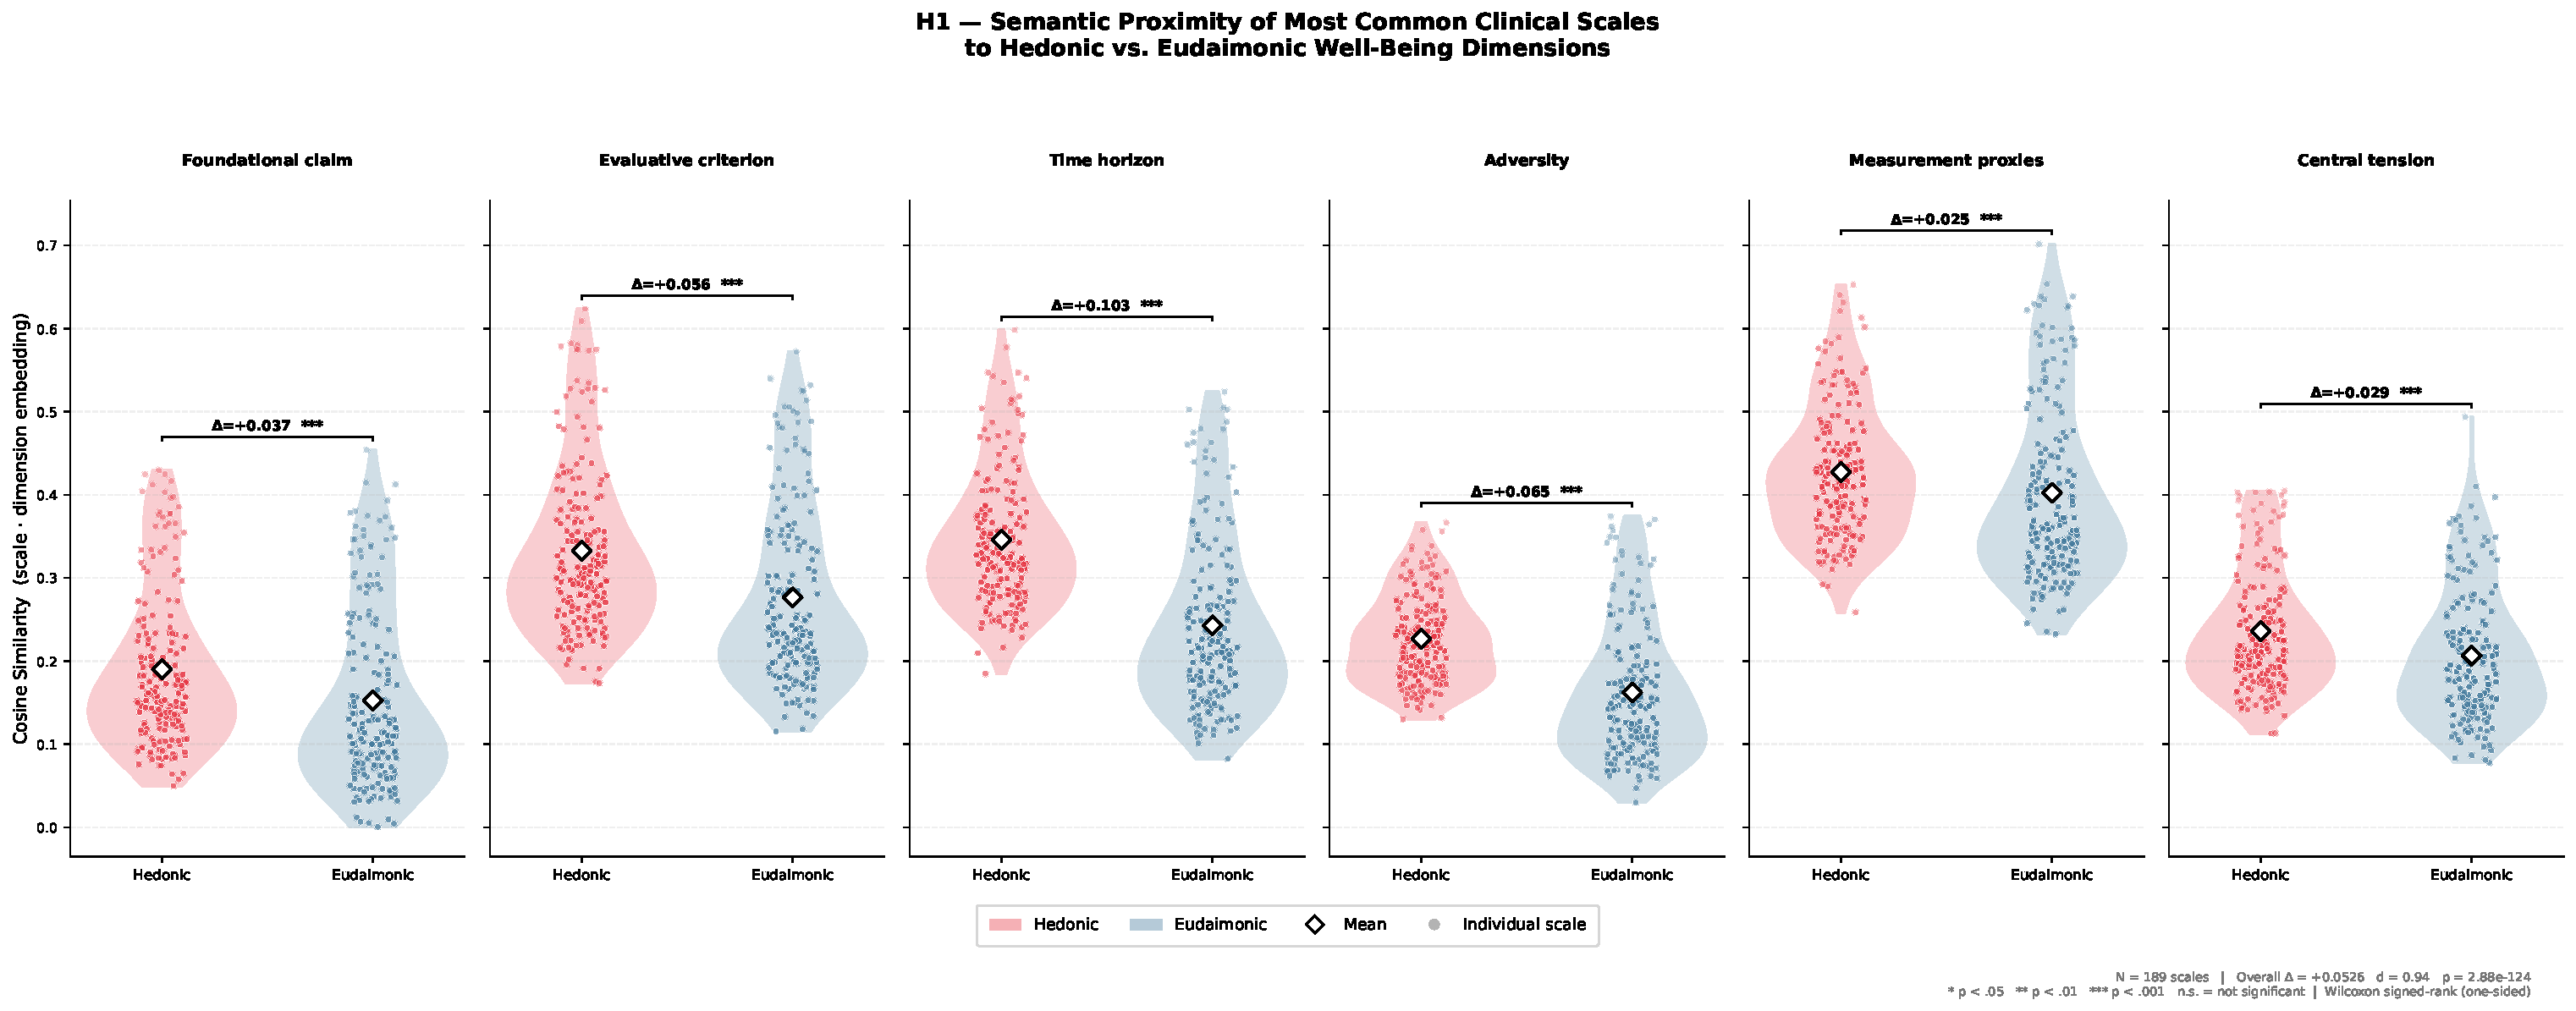
\includegraphics[width=\textwidth]{h1_violin_all.pdf}
    \label{fig:s_unweighted}
    \floatnote{Diamonds represent arithmetic (unweighted) means. Red = hedonic pole; blue = eudaimonic pole. All differences significant at $p < .001$ (Holm-corrected). Raw $\Delta = +0.053$, $d = 0.94$.}
\end{figure}

\clearpage
\subsection*{S2.\ Violin Plots for Top-50 Most-Cited Scales}

\begin{figure}[H]
    \centering
    \caption{Hedonic versus eudaimonic cosine similarities for the 50 most-cited clinical scales (unweighted)}
    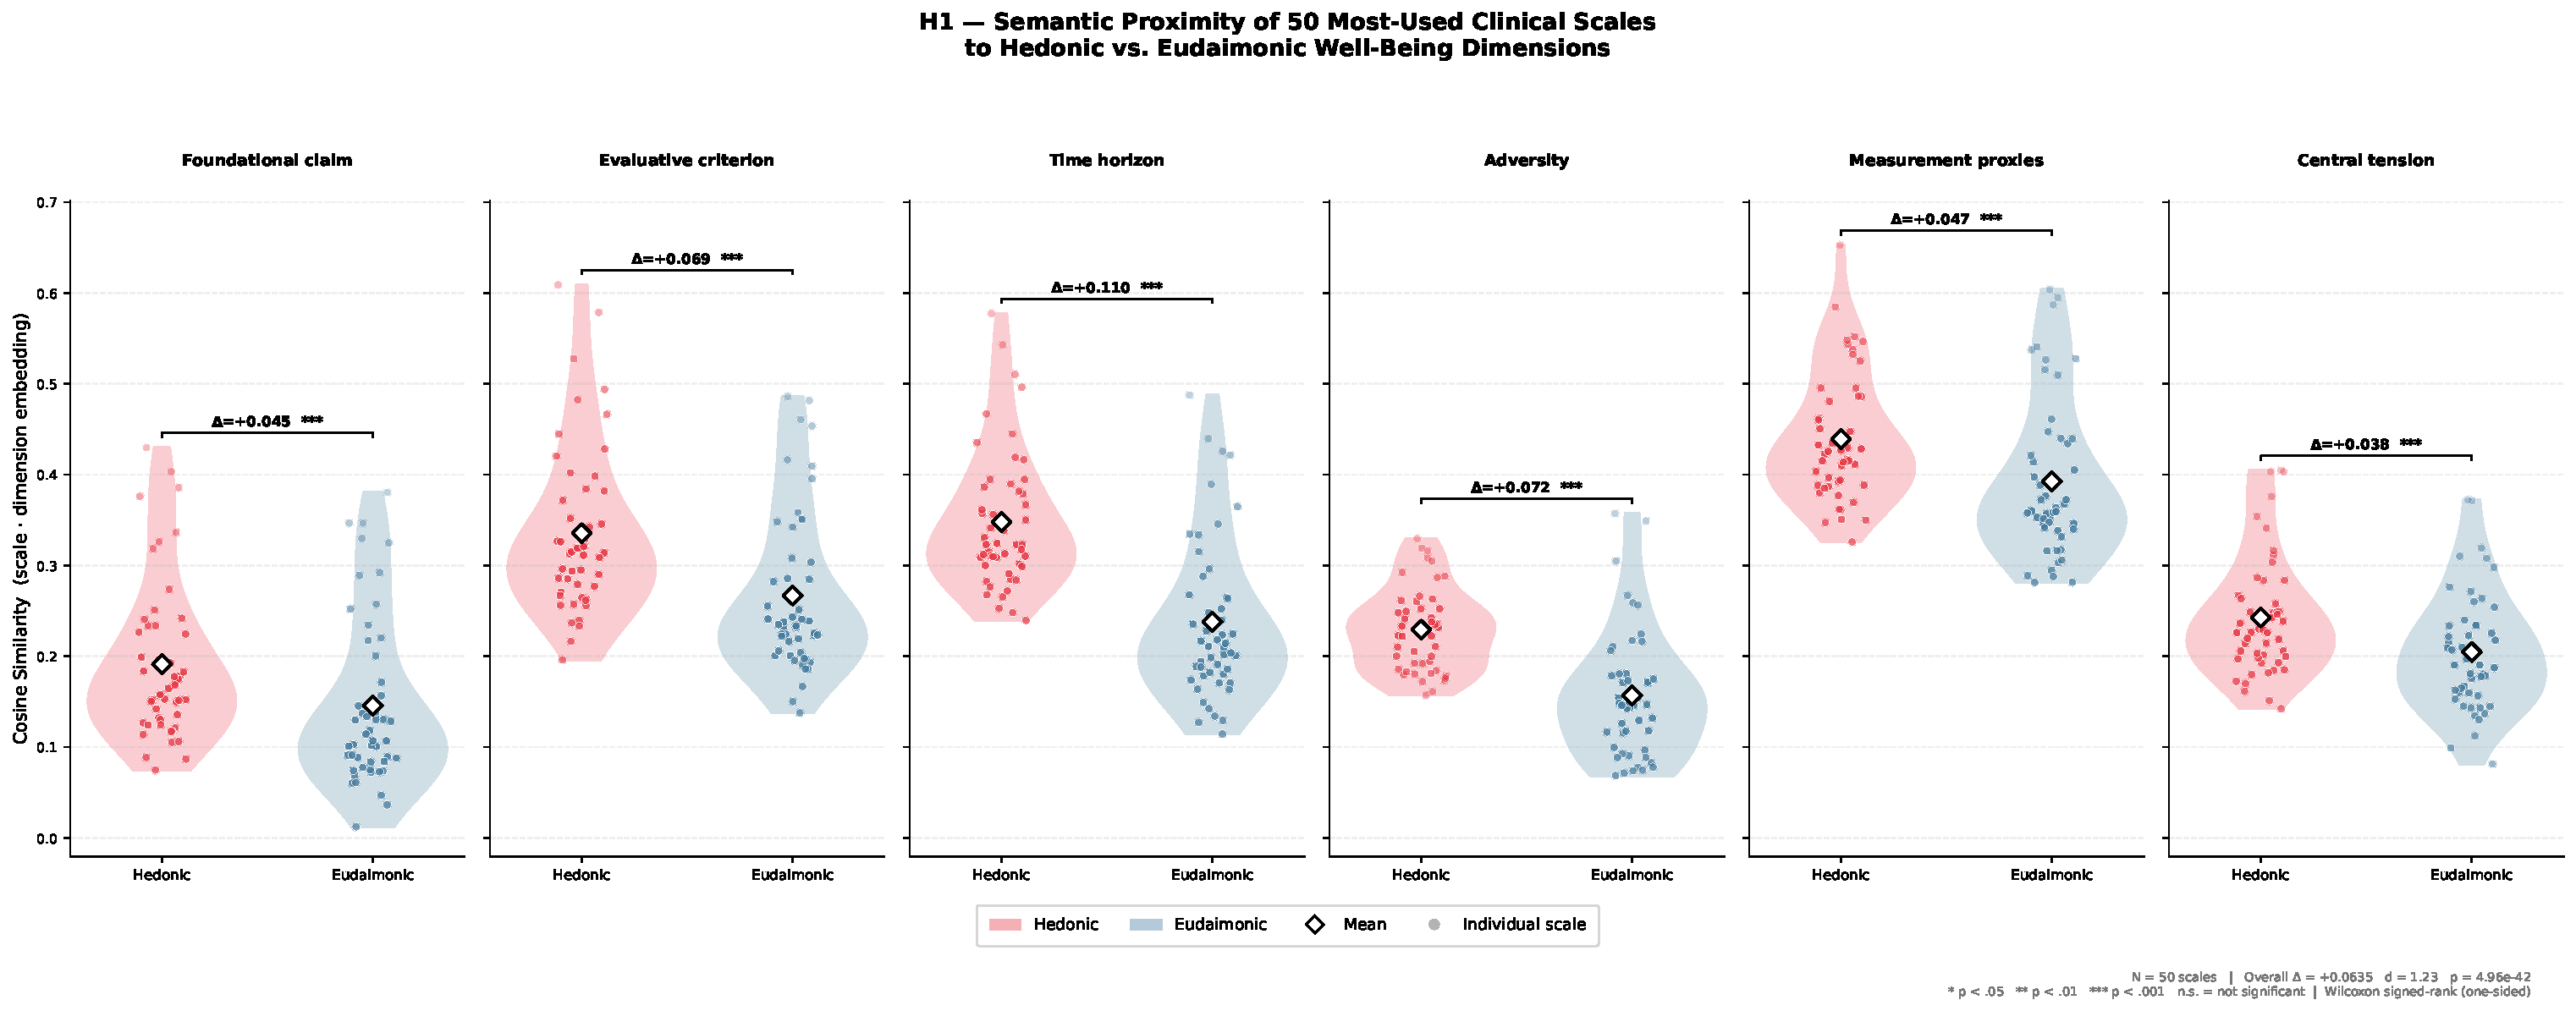
\includegraphics[width=\textwidth]{h1_violin_top50.pdf}
    \label{fig:s_top50}
\floatnote{The hedonic bias is similar in magnitude to the full corpus ($d = 1.23$ vs.\ $d = 0.94$), indicating that citation frequency does not substantially amplify the imbalance.}
\end{figure}

\begin{figure}[H]
    \centering
    \caption{Usage-weighted violin plot for the 50 most-cited clinical scales}
    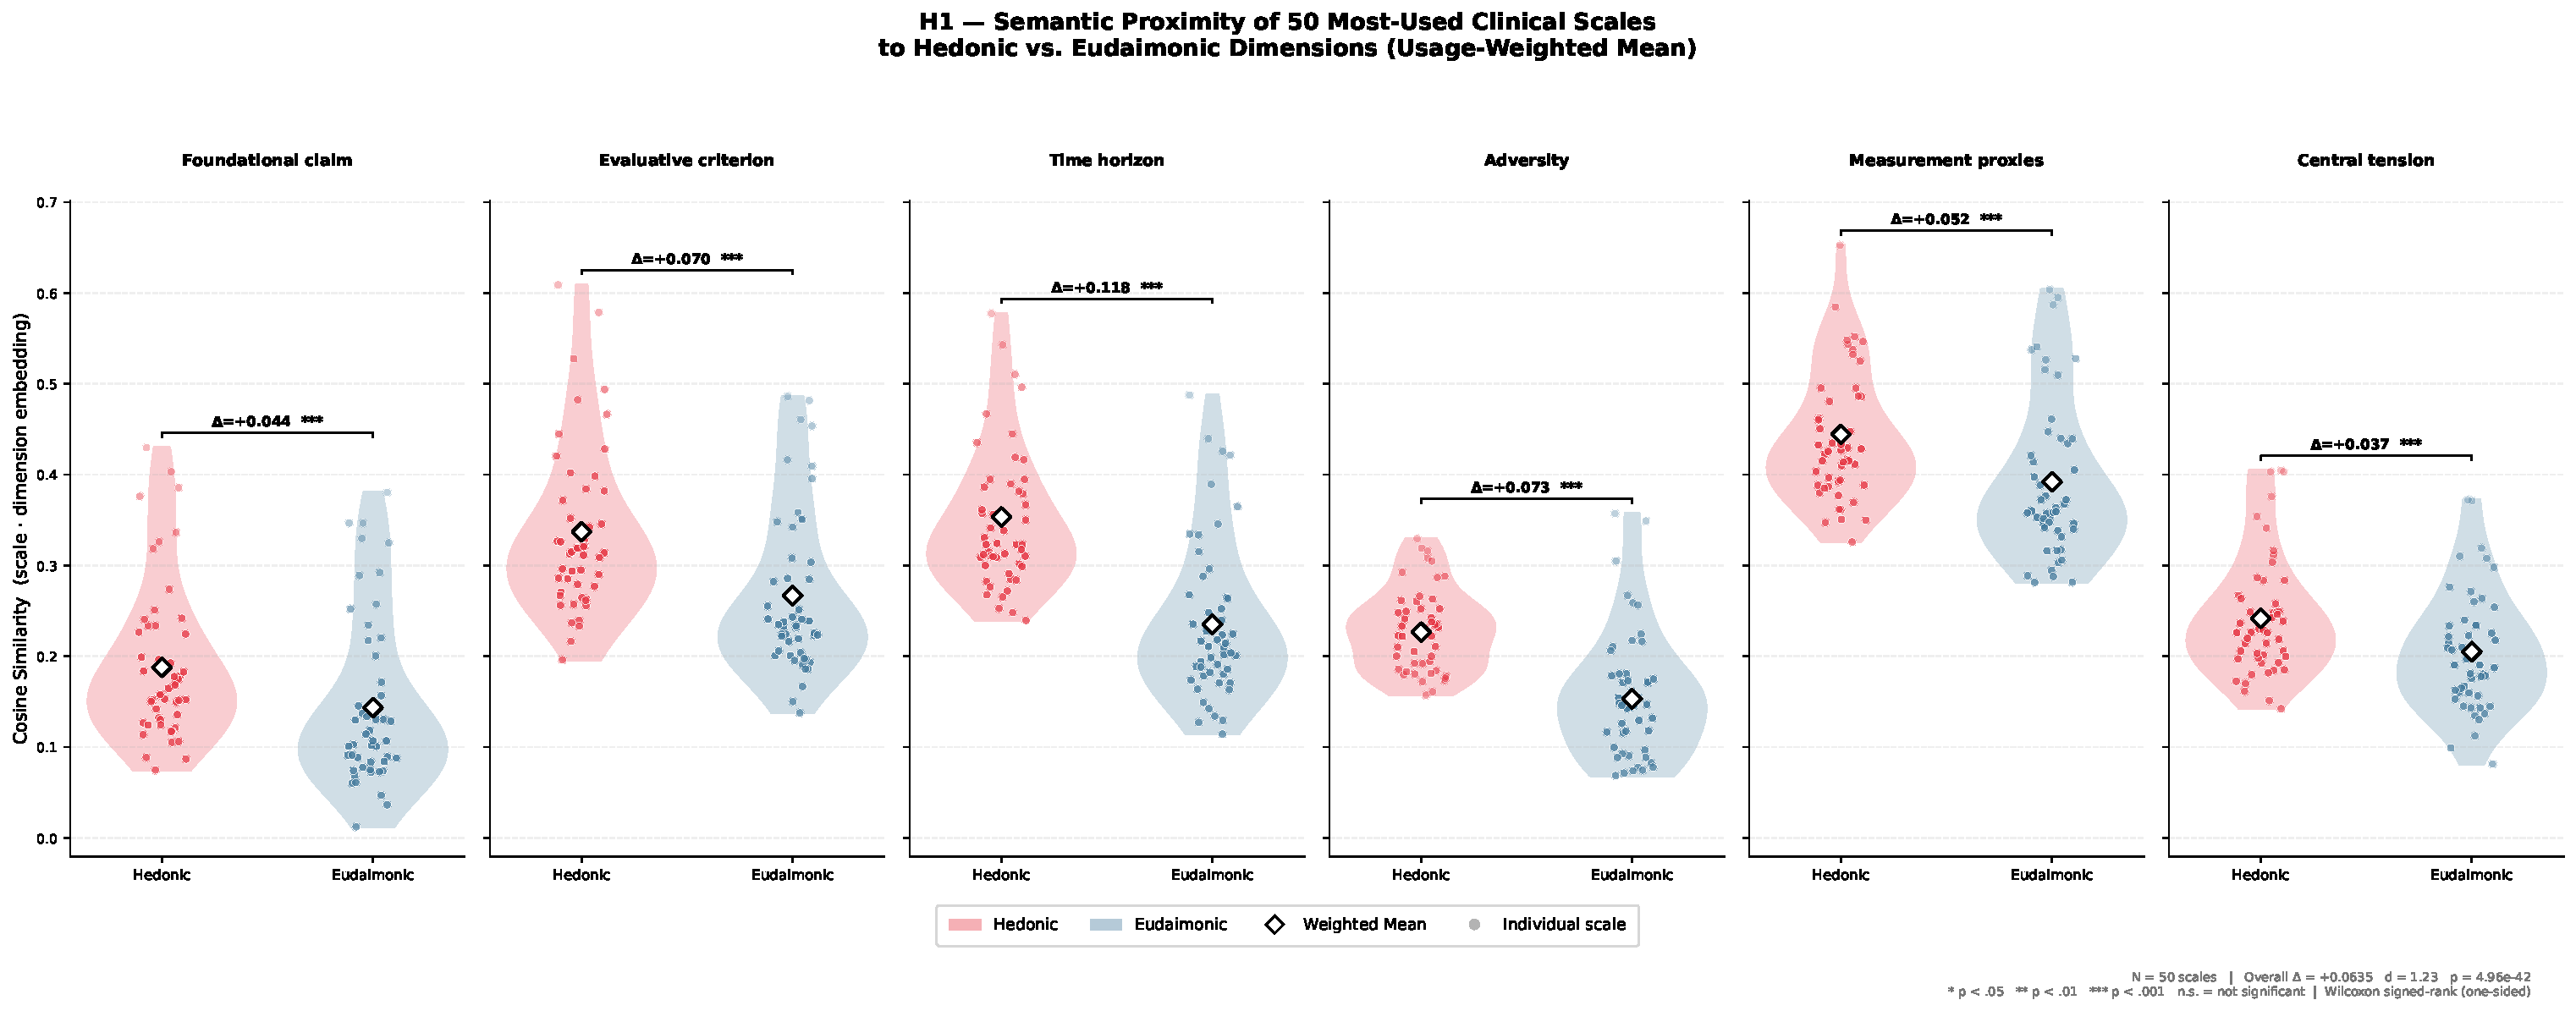
\includegraphics[width=\textwidth]{h1_violin_top50_weighted.pdf}
    \label{fig:s_top50_weighted}
    \floatnote{Diamonds indicate usage-weighted means (weighted $\Delta = +0.066$, $d = 1.36$).}
\end{figure}

\clearpage
\subsection*{S3.\ Four-Panel Comparison of All Sub-Analyses}

\begin{figure}[H]
    \centering
    \caption{Four-panel comparison of all H1 sub-analyses}
    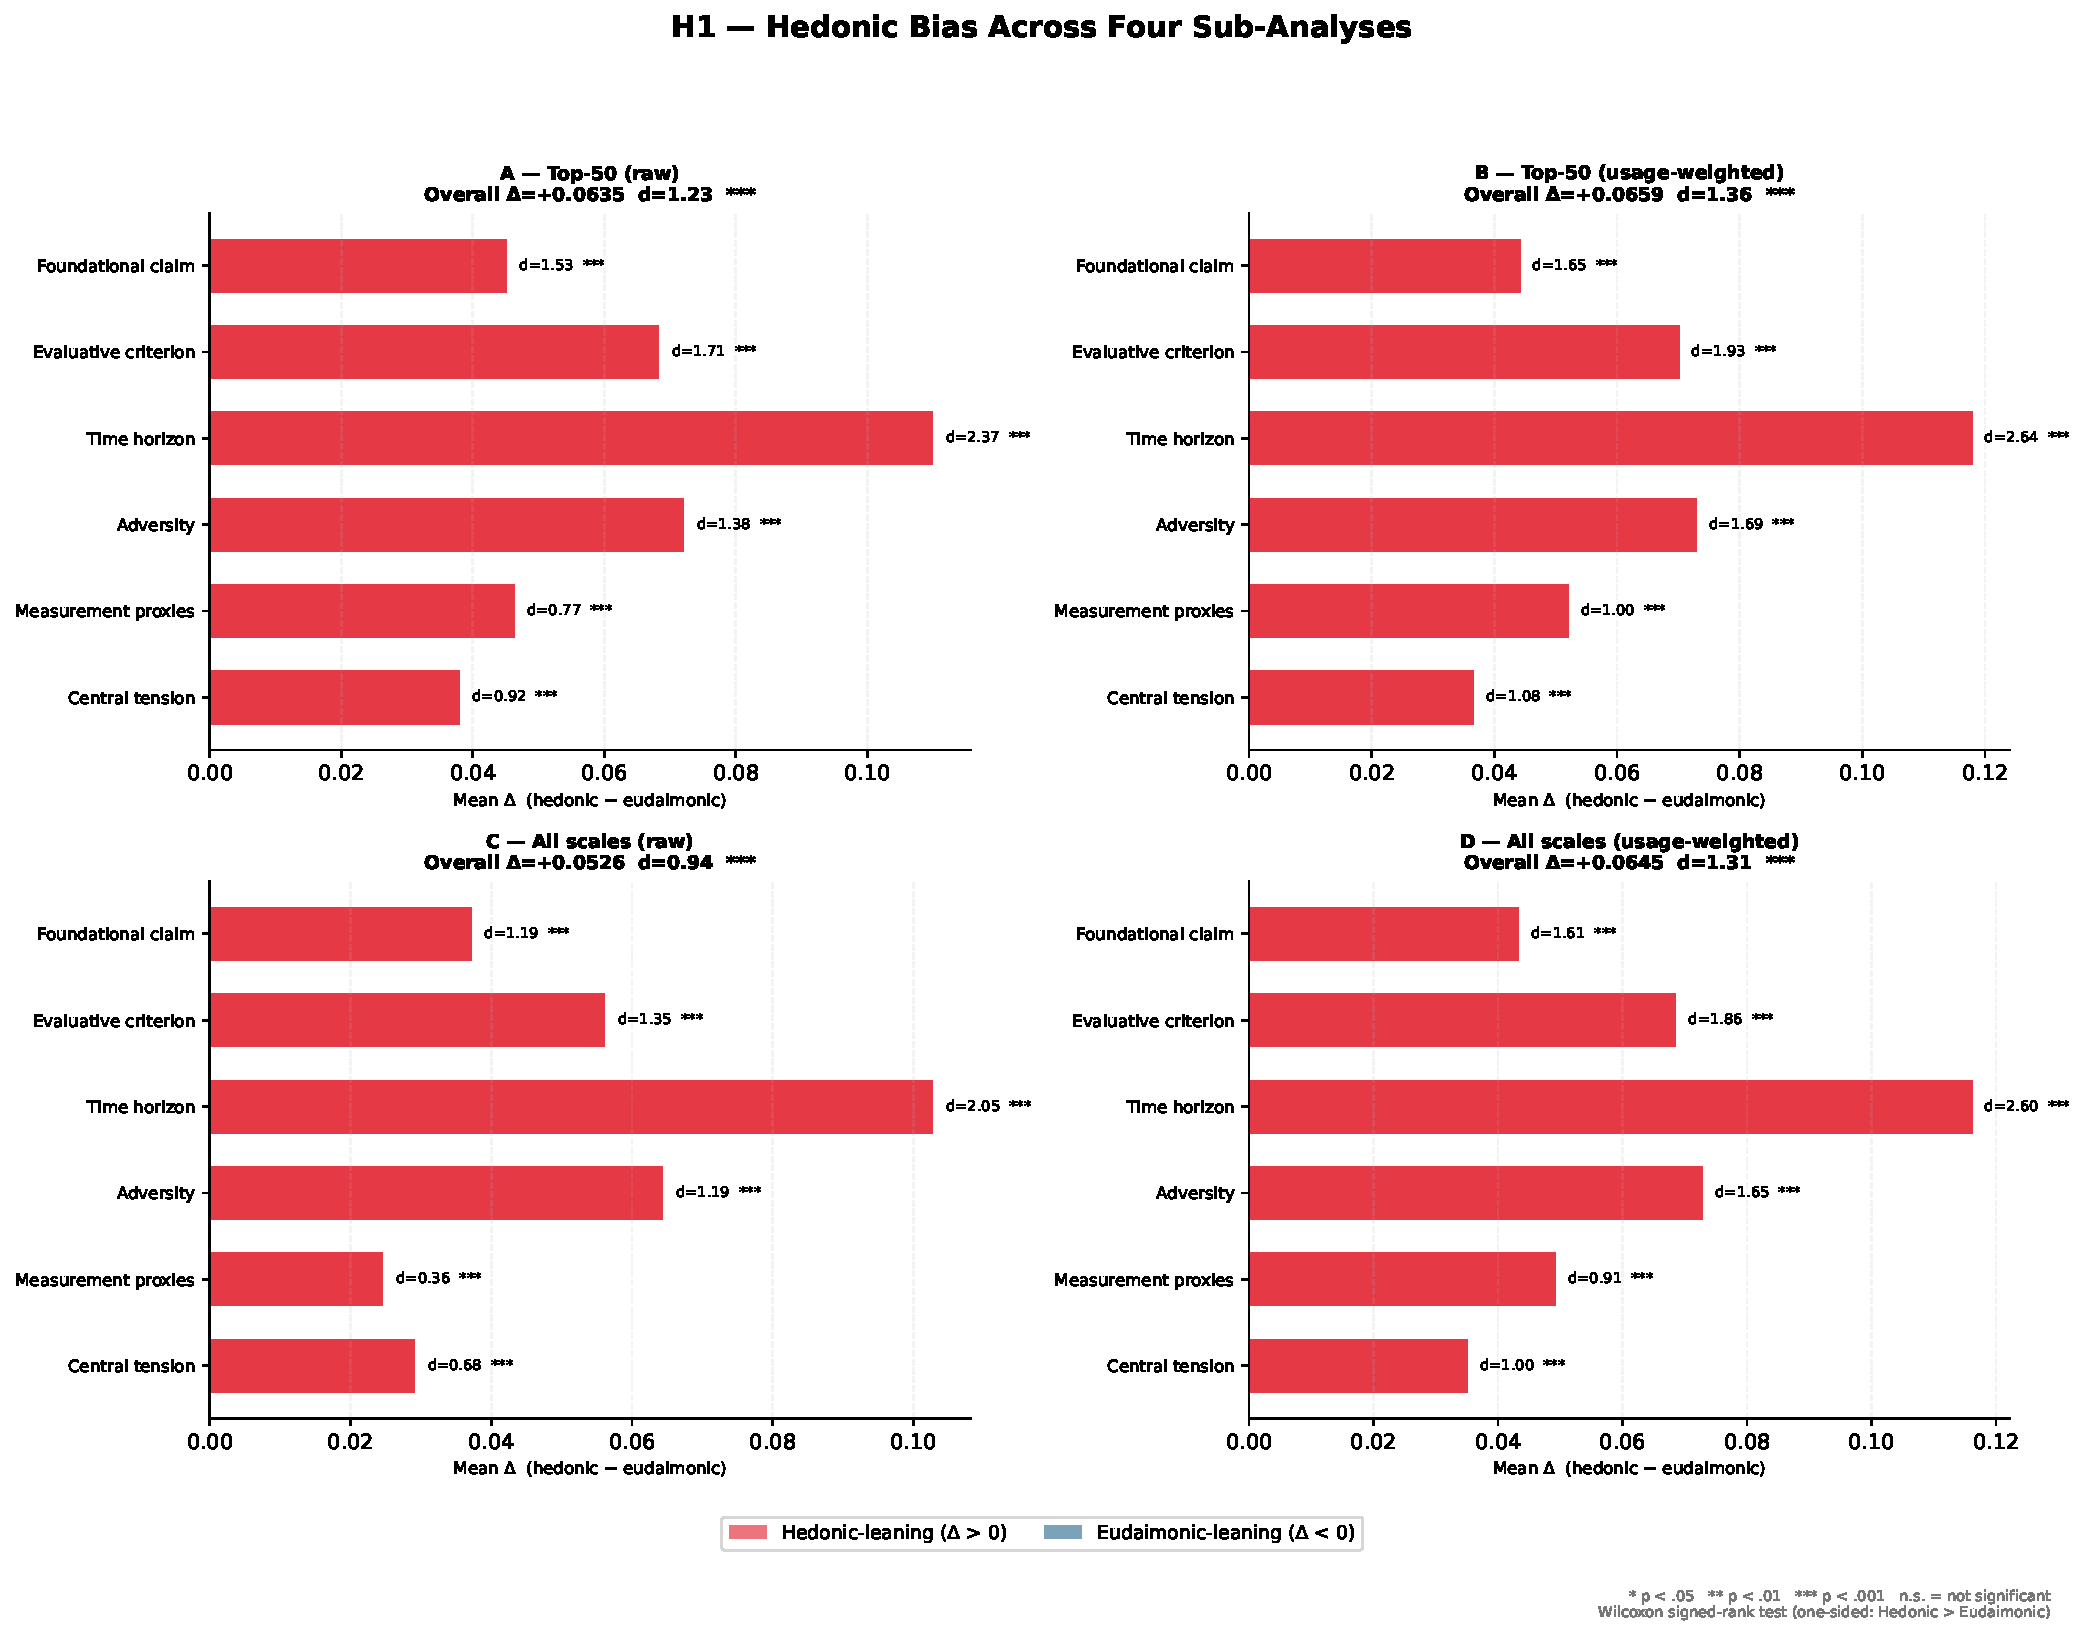
\includegraphics[width=\textwidth]{h1_four_panel.pdf}
    \label{fig:s_four_panel}
    \floatnote{Per-dimension mean $\Delta$ and Cohen's $d$ for all four H1 sub-analyses: (A) Top-50 raw, (B) Top-50 usage-weighted, (C) All scales raw, (D) All scales usage-weighted.}
\end{figure}

\clearpage
\subsection*{S4.\ Effect-Size Comparison}

\begin{figure}[H]
    \centering
    \caption{Cohen's $d$ by dimension across all four sub-analyses}
    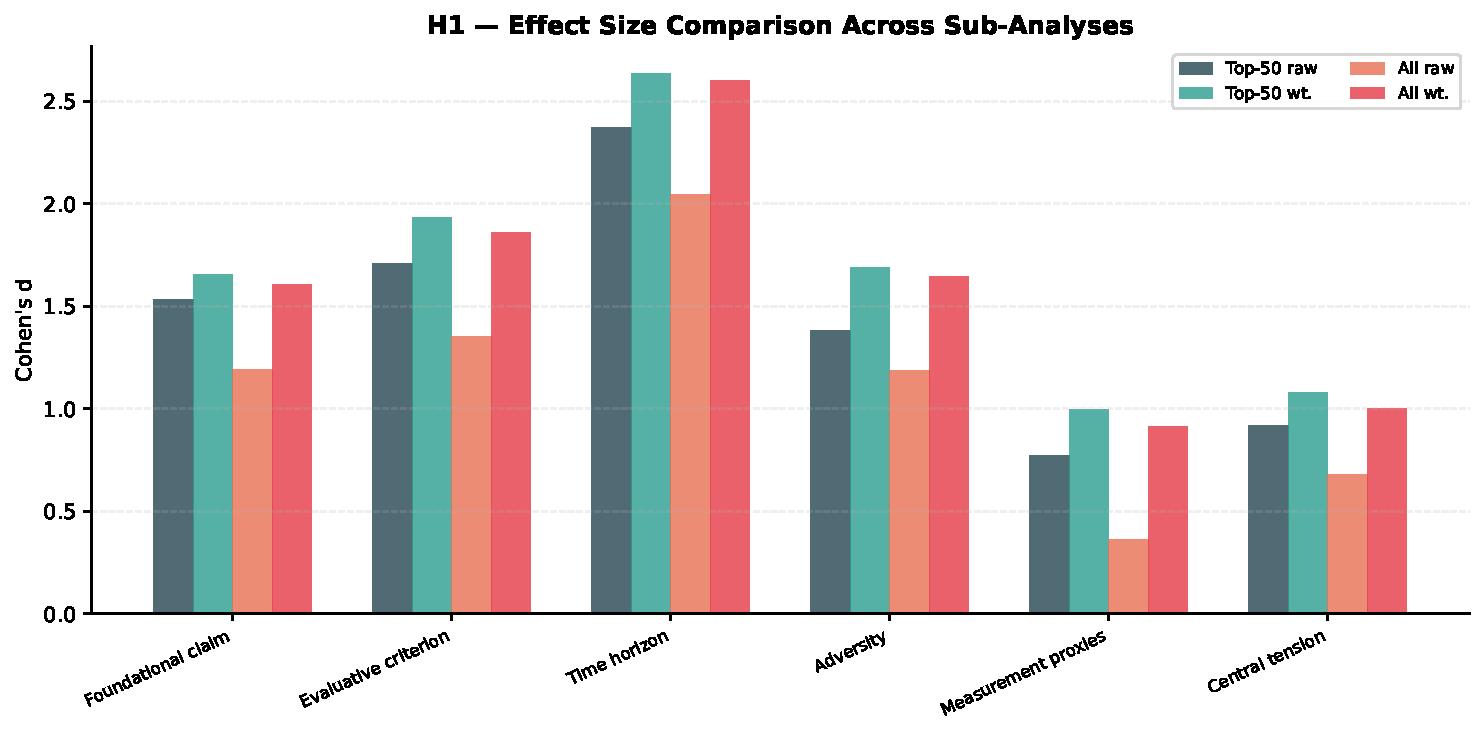
\includegraphics[width=\textwidth]{h1_effect_sizes.pdf}
    \label{fig:s_effect_sizes}
    \floatnote{The consistent pattern across raw and weighted analyses, and across top-50 and full corpus, indicates the hedonic bias is not driven by a few outlier scales.}
\end{figure}

\clearpage
\subsection*{S5.\ Permutation Null Distribution}

\begin{figure}[H]
    \centering
    \caption{Permutation null distribution for the overall hedonic-bias test}
    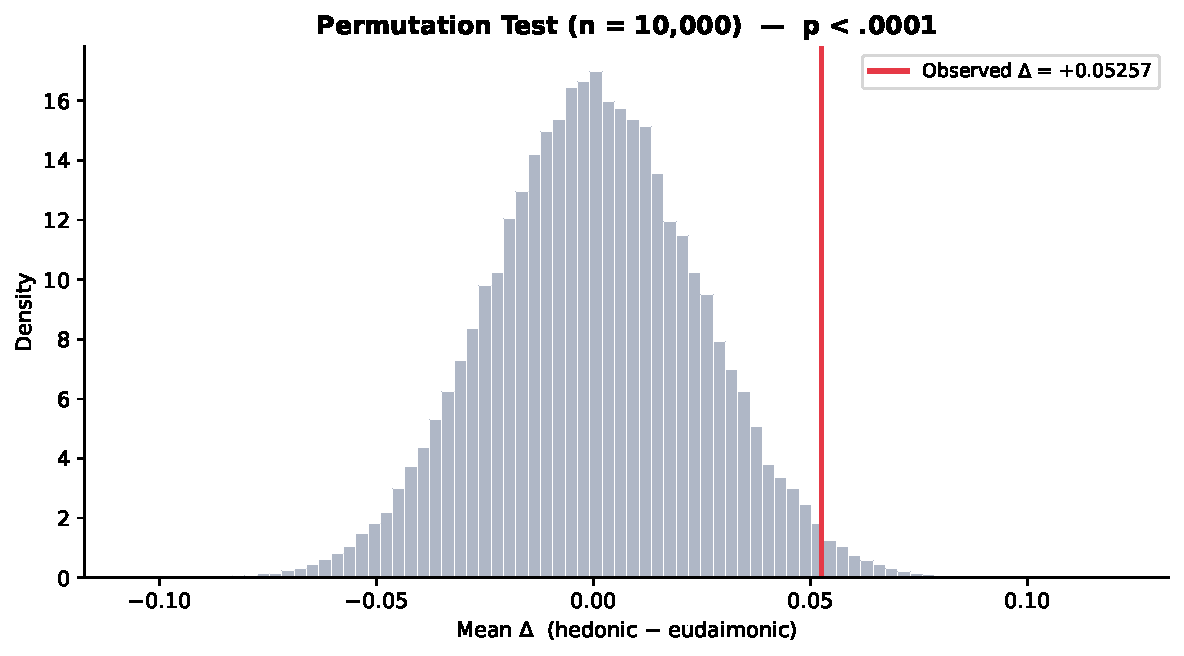
\includegraphics[width=0.75\textwidth]{posthoc_permutation.pdf}
    \label{fig:s_permutation}
    \floatnote{Distribution of mean $\Delta$ under 10,000 random permutations of hedonic and eudaimonic pole labels. The observed $\Delta = +0.053$ (red dashed line) falls far outside the null distribution ($p < .0001$, one-sided).}
\end{figure}

\clearpage
\subsection*{S6.\ Scales with Strongest Hedonic Loading}

Table~\ref{tab:s_top_hedonic} presents the 10 clinical scales with the largest mean $\Delta$ (strongest hedonic loading) across all six dimensions, alongside the 10 scales with the strongest eudaimonic loading. Figure~\ref{fig:s_top10_trends} shows the PubMed publication trajectories (2000--2025) for these two groups.

\begin{table}[H]
\caption{Scales with strongest hedonic and eudaimonic semantic loading}
\label{tab:s_top_hedonic}
\small
\begin{tabular}{rlcrlc}
\toprule
\textbf{Rank} & \textbf{Scale (Hedonic)} & \textbf{Mean $\Delta$} & \textbf{Rank} & \textbf{Scale (Eudaimonic)} & \textbf{Mean $\Delta$} \\
\midrule
 1 & PANAS           & $+0.124$ &  1 & PGI             & $-0.083$ \\
 2 & PHQ-15          & $+0.116$ &  2 & PGIS-II         & $-0.078$ \\
 3 & ZSAS            & $+0.116$ &  3 & VIA-IS          & $-0.077$ \\
 4 & BAI             & $+0.115$ &  4 & ILS             & $-0.069$ \\
 5 & PHQ-2           & $+0.114$ &  5 & RYFF-PWB        & $-0.067$ \\
 6 & DASS-21         & $+0.110$ &  6 & ACT             & $-0.062$ \\
 7 & HAM-A           & $+0.109$ &  7 & GRIT-S          & $-0.049$ \\
 8 & MFQ             & $+0.108$ &  8 & BIEPS           & $-0.043$ \\
 9 & DASS-42         & $+0.107$ &  9 & FLCS            & $-0.033$ \\
10 & PHQ-9           & $+0.107$ & 10 & SBI             & $-0.033$ \\
\bottomrule
\end{tabular}
\floatnote{Mean $\Delta$ averaged across all six hedonic--eudaimonic dimensions. Positive values indicate hedonic orientation; negative values indicate eudaimonic orientation. PGI = Personal Growth Initiative Scale.}
\end{table}

\clearpage

\begin{figure}[H]
\caption{PubMed publication trends (2000--2025) for the 10 scales with the strongest hedonic and eudaimonic loading: raw counts and baseline-corrected ratios}
\label{fig:s_top10_trends}
\centering
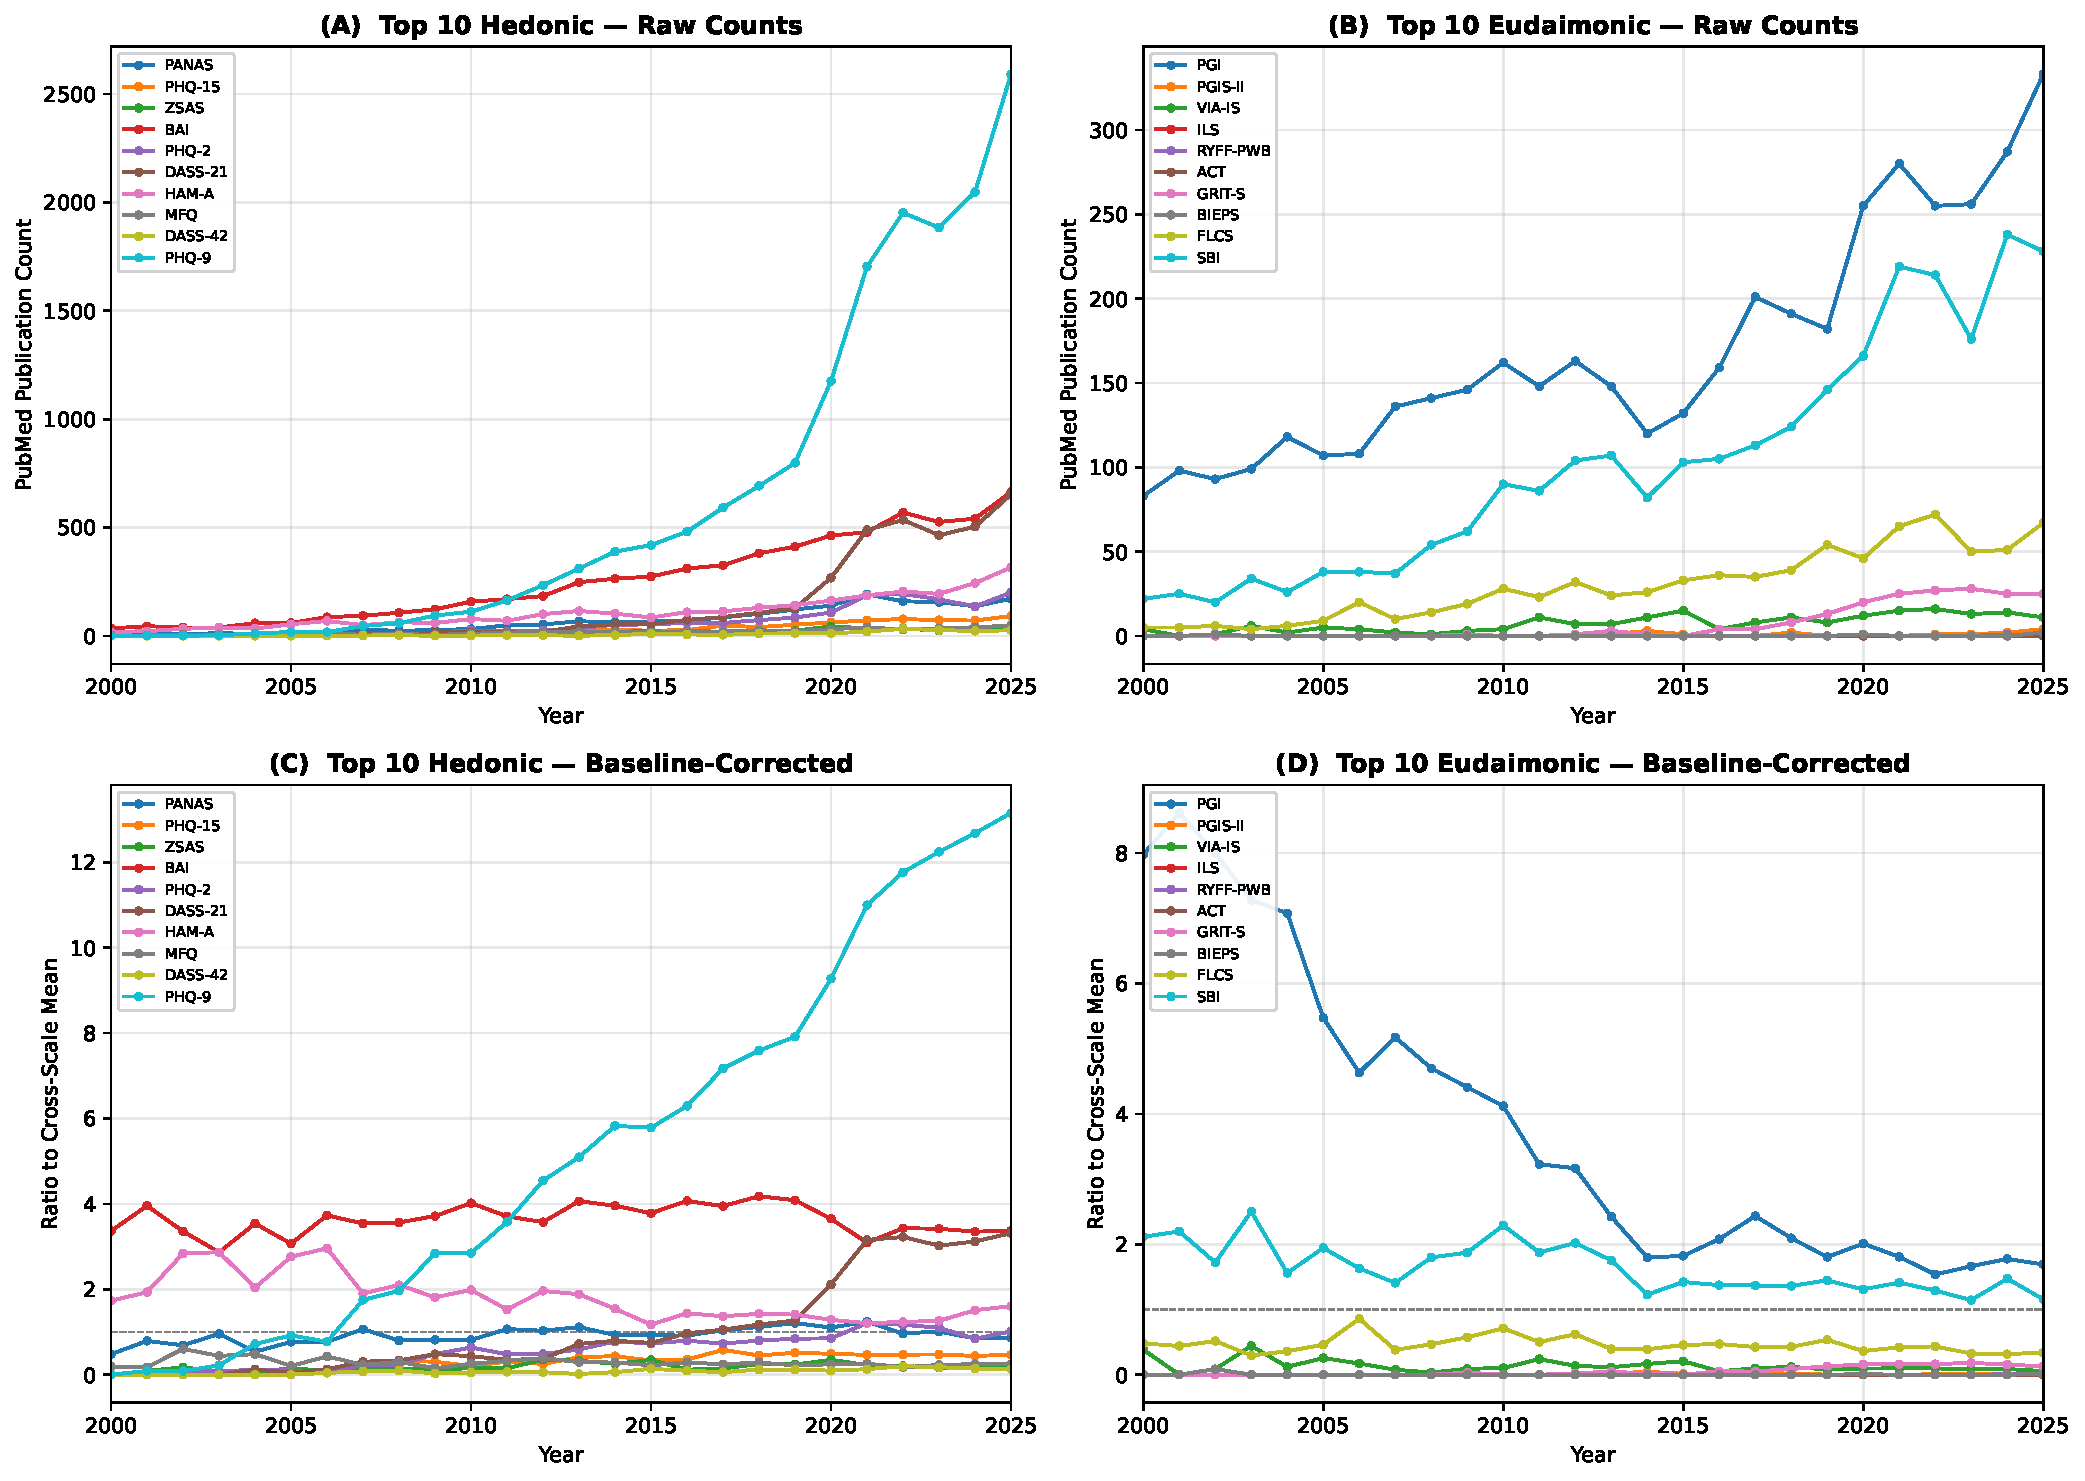
\includegraphics[width=\textwidth]{s_top10_pubmed_trends}
\floatnote{(A)~Raw annual PubMed publication counts for the 10 clinical scales with the largest positive mean~$\Delta$ (hedonic loading). (B)~Raw annual counts for the 10 scales with the most negative mean~$\Delta$ (eudaimonic loading). (C,~D)~Baseline-corrected versions of panels~A and~B. For each year, each scale's count is divided by the cross-scale mean of all 189 scales in that year, yielding a ratio relative to the ``average'' scale (dashed grey line at 1.0). This removes the general upward trend in PubMed publications and isolates relative growth. Hedonic-loaded scales (e.g., PANAS, BAI, PHQ-9) show substantially higher and steeper raw growth compared with eudaimonic-loaded scales (e.g., PGI, VIA-IS, RYFF-PWB); however, both groups converge toward the cross-scale mean after baseline correction, indicating that absolute differences in adoption---rather than differential growth rates---drive the usage-weighted bias reported in H1.}
\end{figure}

\clearpage
\subsection*{S7.\ Per-Dimension Embedding Similarity Summary Statistics}

\begin{table}[H]
\caption{Descriptive statistics of cosine similarities by dimension and pole (all 189 scales)}
\label{tab:s_dim_descriptives}
\small
\begin{tabular}{lcccccc}
\toprule
 & \multicolumn{3}{c}{\textbf{Hedonic Similarity}} & \multicolumn{3}{c}{\textbf{Eudaimonic Similarity}} \\
\cmidrule(lr){2-4} \cmidrule(lr){5-7}
\textbf{Dimension} & \textbf{Mean} & \textbf{SD} & \textbf{Range} & \textbf{Mean} & \textbf{SD} & \textbf{Range} \\
\midrule
Foundational claim        & 0.190 & 0.094 & [0.05, 0.43] & 0.153 & 0.107 & [0.00, 0.45] \\
Evaluative criterion      & 0.333 & 0.101 & [0.17, 0.62] & 0.276 & 0.108 & [0.12, 0.57] \\
Time horizon              & 0.346 & 0.082 & [0.19, 0.60] & 0.243 & 0.103 & [0.08, 0.52] \\
Adversity                 & 0.227 & 0.053 & [0.13, 0.37] & 0.162 & 0.081 & [0.03, 0.37] \\
Measurement proxies       & 0.427 & 0.079 & [0.26, 0.65] & 0.402 & 0.106 & [0.23, 0.70] \\
Central tension           & 0.236 & 0.071 & [0.11, 0.40] & 0.207 & 0.080 & [0.08, 0.49] \\
\bottomrule
\end{tabular}
\floatnote{Values are cosine similarities between scale embeddings and each pole. Ranges show [minimum, maximum] across all 189 scales.}
\end{table}

\clearpage
\subsection*{S8.\ Twenty Most-Used Clinical Scales}

\begin{table}[H]
\caption{Twenty most-used clinical scales by cumulative PubMed publication count (2000--2025)}
\label{tab:s_top_usage}
\small
\begin{tabularx}{\textwidth}{rlXlrc}
\toprule
\textbf{Rank} & \textbf{Abbrev.} & \textbf{Full Name} & \textbf{Domain} & \textbf{Pubs} & \textbf{Mean $\Delta$} \\
\midrule
 1 & PSS & Perceived Stress Scale & Anxiety & 24,152 & $+0.076$ \\
 2 & PHQ-9 & Patient Health Questionnaire-9 & Mood & 15,799 & $+0.107$ \\
 3 & PSQI & Pittsburgh Sleep Quality Index & Functional & 14,855 & $+0.080$ \\
 4 & EQ-5D & EuroQol Five Dimensions & Functional & 19,272 & $+0.063$ \\
 5 & SCS & Self-Compassion Scale & Eudaimonic & 17,825 & $+0.019$ \\
 6 & RRS & Ruminative Responses Scale & Mood & 17,700 & $+0.046$ \\
 7 & GAD-7 & Generalized Anxiety Disorder 7-item Scale & Anxiety & 6,343 & $+0.087$ \\
 8 & PROMIS & Patient-Reported Outcomes Measurement Information System & Functional & 7,758 & $+0.062$ \\
 9 & MBI & Maslach Burnout Inventory & General Distr. & 7,826 & $+0.025$ \\
10 & STAI & State-Trait Anxiety Inventory & Anxiety & 9,935 & $+0.077$ \\
11 & MFI & Multidimensional Fatigue Inventory & Functional & 7,259 & $+0.038$ \\
12 & BAI & Beck Anxiety Inventory & Anxiety & 6,657 & $+0.115$ \\
13 & EPDS & Edinburgh Postnatal Depression Scale & Mood & 6,237 & $+0.098$ \\
14 & DASS-21 & Depression Anxiety Stress Scales-21 & General Distr. & 3,553 & $+0.110$ \\
15 & SF-12 & Short Form Health Survey-12 & Functional & 8,232 & $+0.042$ \\
16 & QOLS & Quality of Life Scale & Eudaimonic & 5,070 & $+0.038$ \\
17 & EPOCH & EPOCH Measure of Adolescent Well-Being & Eudaimonic & 6,286 & $-0.025$ \\
18 & WHOQOL-BREF & World Health Organization Quality of Life-BREF & Functional & 4,956 & $+0.057$ \\
19 & SDQ & Strengths and Difficulties Questionnaire & General Distr. & 5,538 & $+0.071$ \\
20 & BDI-II & Beck Depression Inventory-II & Mood & 5,932 & $+0.102$ \\
\bottomrule
\end{tabularx}
\floatnote{Cumulative PubMed publications (2000--2025). Usage weights normalised to sum to 1.0 across all 189 scales. Mean $\Delta$ averaged across all six hedonic--eudaimonic dimensions. 20 of 20 most-used scales show positive (hedonic) loading.}
\end{table}

\clearpage
\subsection*{S9.\ Mental-Health Book Replication of H1 (Cross-Sectional Hedonic Bias)}
\label{sec:s_ngram_h1}

\subsubsection*{Method}

To test whether the hedonic loading observed in clinical scales reflects a broader asymmetry in evaluative language within mental-health literature---rather than a property unique to psychometric instruments---we conducted a convergent-validity replication using word frequencies drawn from a large corpus of psychology and psychiatry books.

\paragraph{Corpus construction.}
We constructed a domain-restricted corpus from the Internet Archive, a digital library containing over 40~million items with structured subject metadata.
We searched for English-language items classified under psychology, psychiatry, mental health, psychotherapy, clinical psychology, psychopathology, abnormal psychology, behavioural sciences, psychometrics, counselling psychology, cognitive therapy, or psychological assessment.
To ensure temporal coverage, we stratified the search by decade (1900s--2010s), retrieving up to 500 books per decade sorted by download count (a proxy for scholarly relevance).
Because recent decades had sparser initial coverage, we augmented the corpus with additional broad queries (title-based and publisher-based searches for clinical-psychology, psychiatry, and psychotherapy content), again stratified by decade and filtered to mental-health subjects.
The combined candidate set comprised approximately 16{,}000 unique volumes.

\paragraph{Text extraction.}
For each candidate volume, we attempted to download the OCR text file (\texttt{\_djvu.txt} or \texttt{.txt}) from the Internet Archive.
Books behind access restrictions (e.g., controlled digital lending for copyrighted works) returned HTTP~401 and were excluded.
Texts with fewer than 500 tokens after tokenisation were discarded as pamphlets or fragments.
This procedure yielded 3{,}883 successfully processed books spanning 1900--2019, with the strongest representation in the pre-copyright era (1900--1929: $\sim$1{,}460 books) and improved coverage in recent decades (2000--2019: 259~books) following the augmentation step.

\paragraph{Word frequency extraction.}
Each book was tokenised using a simple alphabetic regex (words $\geq 3$ characters), lowercased, and matched against the 9{,}288-word vocabulary of high-frequency English adjectives and verbs established from the Google Books Ngram pipeline (Section~2.5.3).
This intersection ensures that (a)~all counted words have pre-computed embeddings, and (b)~the word set is identical across all analyses, enabling direct comparison.
Word counts were aggregated by (word, year) across all books published in each year, producing a frequency matrix analogous to the Google Books Ngram data but restricted to mental-health literature.
The final dataset comprised 907{,}627 word--year observations across 9{,}286 unique words.

Critically, the filtering occurs at the \textit{book level}---only books whose subject metadata matches mental-health fields are included---not at the word level.
This means the resulting word frequencies reflect natural language use \textit{within} mental-health literature, without any semantic pre-selection of words.

\paragraph{Embedding and similarity computation.}
Identical to the main analysis: each word was embedded using OpenAI \texttt{text-embedding-3-large}, and cosine similarities to the six hedonic--eudaimonic dimension pairs were computed.

\paragraph{Frequency weighting.}
Each word's contribution was weighted by its mean annual frequency over the period 2000--2019 (the most recent decades with sufficient book coverage), normalised to sum to 1.0.

\paragraph{Statistical tests.}
Wilcoxon signed-rank tests (one-sided: hedonic $>$ eudaimonic), frequency-weighted Cohen's $d$, and Holm--Bonferroni correction across six dimensions, identical to the main H1 procedure.

\subsubsection*{Results}

Figure~\ref{fig:s_ngram_h1} presents the distribution of cosine similarities across the six dimensions.
Contrary to the clinical H1 finding, the mental-health book analysis did \textit{not} reveal a hedonic bias.
The overall frequency-weighted $\Delta_w$ was $-0.013$ ($d_w = -0.45$, Wilcoxon $p = 1.0$), indicating that the vocabulary of mental-health literature leans \textit{slightly eudaimonic} rather than hedonic.
All six dimensions yielded negative weighted deltas: Foundational claim ($\Delta_w = -0.003$, $d_w = -0.15$), Evaluative criterion ($\Delta_w = -0.015$, $d_w = -0.68$), Time horizon ($\Delta_w = -0.004$, $d_w = -0.13$), Adversity ($\Delta_w = -0.005$, $d_w = -0.14$), Measurement proxies ($\Delta_w = -0.020$, $d_w = -0.75$), and Central tension ($\Delta_w = -0.034$, $d_w = -1.15$).
After Holm--Bonferroni correction, none of the dimensions reached significance ($p_{\text{adj}} = 1.0$ for all six).
The analysis was based on $N = 9{,}285$ unique words appearing in the mental-health book corpus, yielding 55{,}710 word--dimension similarity pairs.

\begin{figure}[H]
    \centering
    \caption{Mental-health book replication of H1: hedonic versus eudaimonic cosine similarities for 9{,}285 words from 3{,}883 psychology/psychiatry books (frequency-weighted)}
    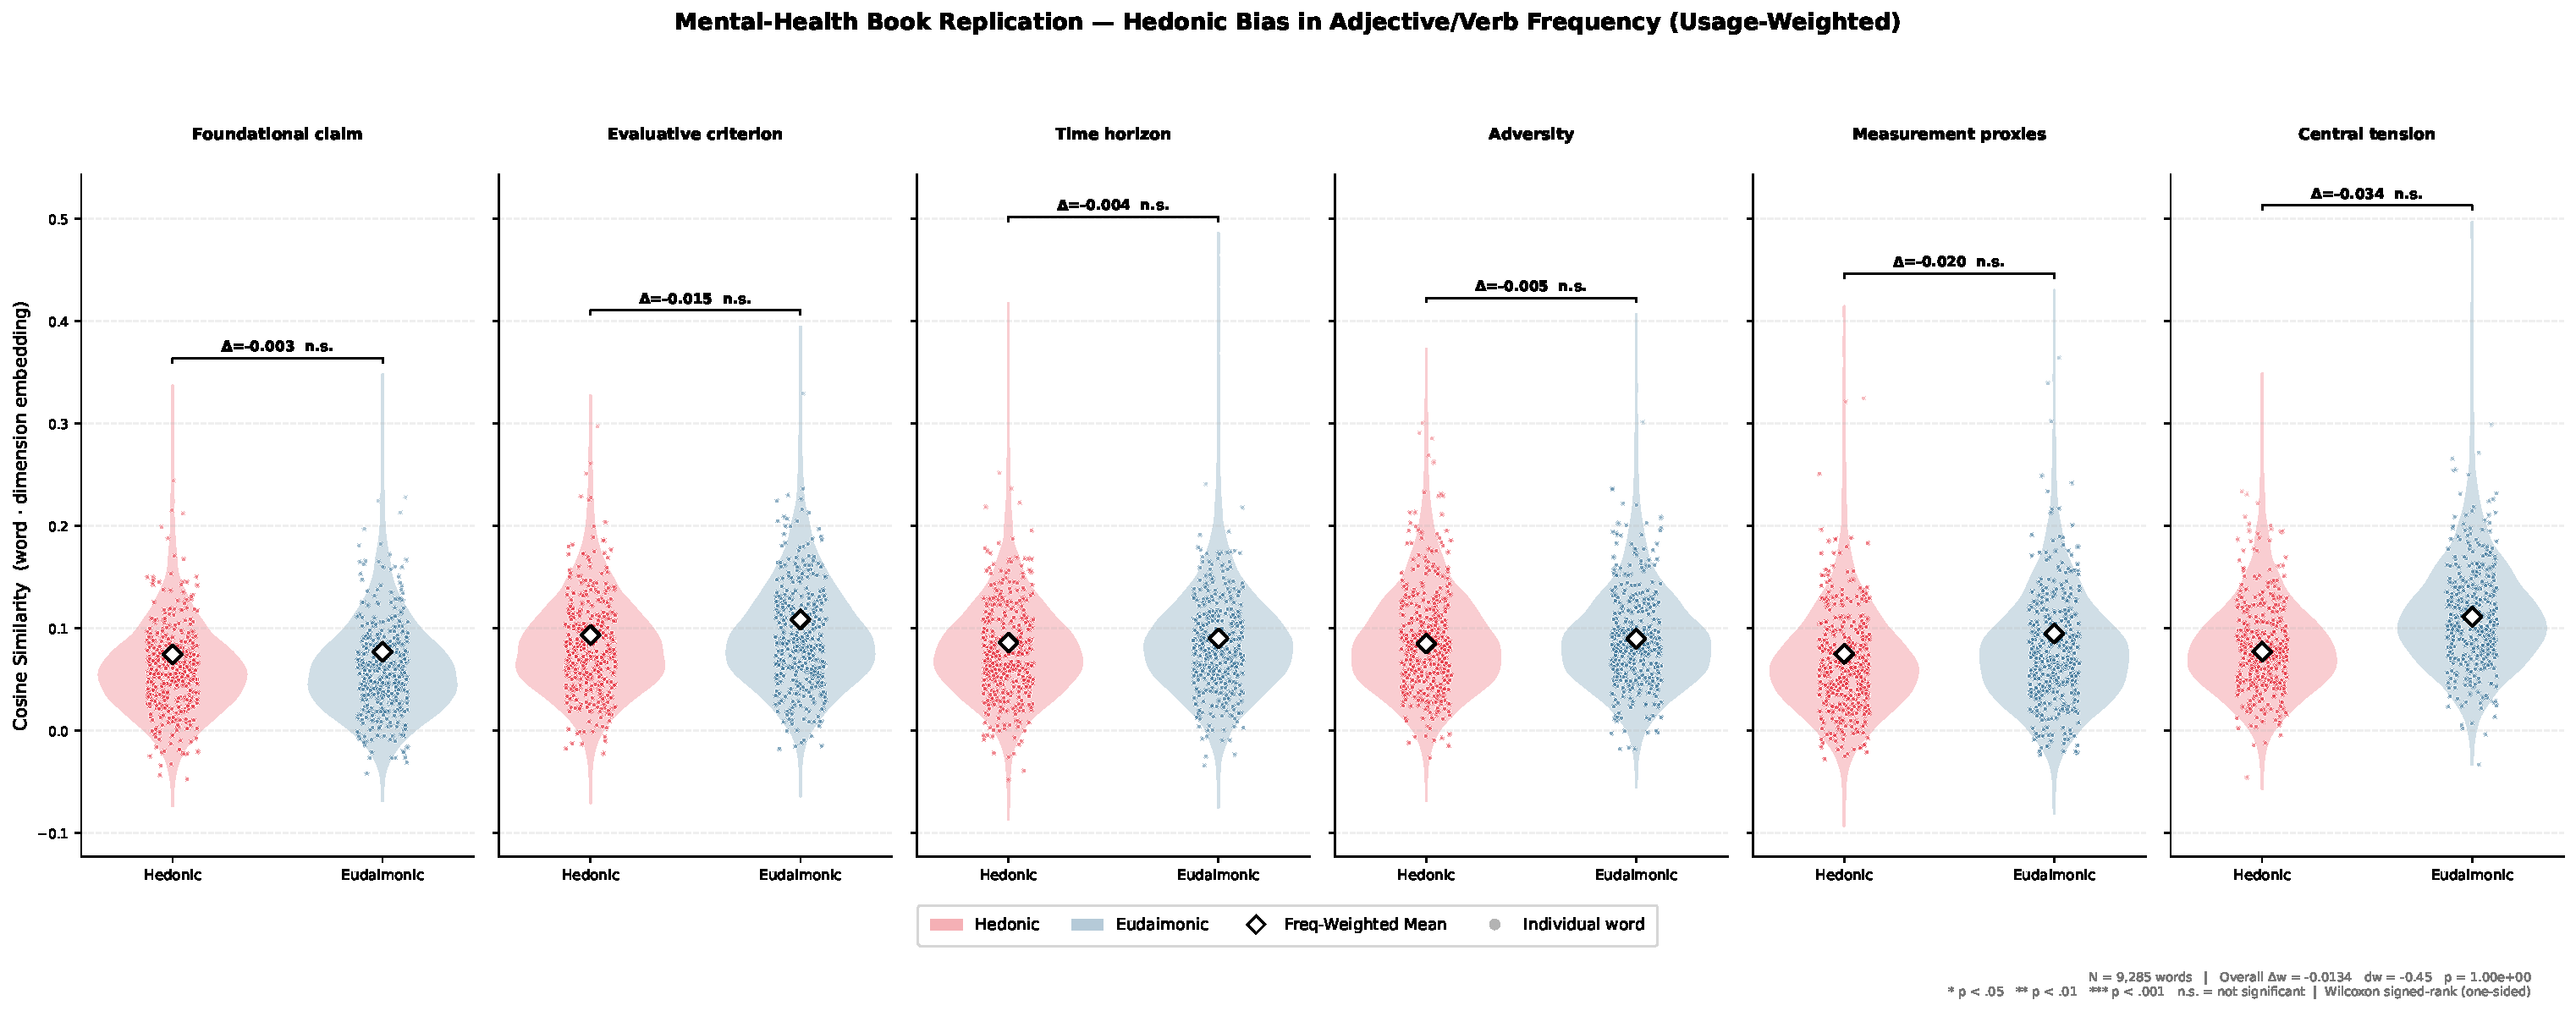
\includegraphics[width=\textwidth]{ngram_h1_violin.pdf}
    \label{fig:s_ngram_h1}
    \floatnote{Distribution of cosine similarities between 9{,}285 words appearing in 3{,}883 Internet Archive mental-health books (1900--2019) and hedonic (red) versus eudaimonic (blue) well-being poles. Diamonds represent frequency-weighted means (2000--2019). No systematic hedonic bias was observed: the overall frequency-weighted $\Delta_w = -0.013$, indicating a slight eudaimonic lean even in mental-health-specific literature. This null finding strengthens the interpretation that the clinical hedonic bias (H1) is specific to psychometric instrumentation rather than a general property of mental-health language.}
\end{figure}

\subsubsection*{Interpretation}

The \textit{absence} of a hedonic bias in mental-health literature is a theoretically informative null finding that sharpens the interpretation of the clinical H1 result in an important way.
Unlike the Google Books Ngram corpus, which spans all literary genres, this corpus was filtered at the book level to include only works classified under psychology, psychiatry, and related mental-health disciplines.
The fact that even this domain-restricted corpus shows no hedonic tilt---and, if anything, leans slightly eudaimonic ($d_w \approx -0.45$)---demonstrates that the clinical bias documented in H1 is \textit{specific to the psychometric measurement ecosystem}, not a property of mental-health vocabulary broadly.

This finding has three key implications.
First, it rules out the possibility that the clinical hedonic bias is an artefact of the embedding model's training data: if the model's distributional semantics inherently favoured hedonic associations, that bias would appear in mental-health literature as well.
Second, psychology and psychiatry as disciplines engage extensively with eudaimonic constructs---meaning, purpose, growth, resilience, character---in their textbooks, theoretical works, and research literature.
The hedonic bias emerges only when this rich conceptual vocabulary is funnelled through the narrow aperture of psychometric instrument design, where RCT methodology, regulatory demands, and psychometric convenience selectively amplify hedonic symptom content.
Third, the larger effect size of the eudaimonic lean in mental-health books ($d_w = -0.44$) compared to general English ($d_w$ in the Google Books analysis) suggests that mental-health literature may be more engaged with eudaimonic themes than general text, making the contrast with the hedonic-biased measurement ecosystem all the more striking.

\clearpage
\subsection*{S10.\ Mental-Health Book Replication of H2 (Temporal Trends in Hedonic Bias)}
\label{sec:s_ngram_h2}

\subsubsection*{Method}

Using the same 3{,}883-book corpus and embedding framework described in Supplementary Note~\ref{sec:s_ngram_h1}, we conducted a temporal replication of H2 spanning 120~years (1900--2019), extending the 25-year clinical temporal analysis to a substantially longer historical window.

\paragraph{Per-year frequency weighting.}
For each year $t \in [1900, 2019]$ and each dimension $d$, we computed the frequency-weighted mean $\Delta$:
\[
\bar{\Delta}_{d,t} = \sum_{w} \omega_{w,t} \cdot \Delta_{w,d}
\]
where $\omega_{w,t}$ is the proportion of word $w$'s frequency in year $t$ relative to the total frequency of all words in that year, as measured in the mental-health book corpus.
An aggregate series was computed by averaging across the six dimensions.
Because each word's embedding is fixed, all temporal variation in $\bar{\Delta}_{d,t}$ reflects shifts in the relative frequency of hedonic versus eudaimonic vocabulary within mental-health texts---i.e., which words are used more or less often---rather than changes in word meaning.

\paragraph{Trend statistics.}
Identical to the main H2 procedure: ordinary least-squares (OLS) regression on year, 10{,}000-fold bootstrap confidence intervals on the slope, Mann-Kendall test for monotonic trend, and Durbin--Watson diagnostics for residual autocorrelation.

\subsubsection*{Results}

Figure~\ref{fig:s_ngram_h2} presents the temporal evolution of frequency-weighted $\Delta$ across the six dimensions and the aggregate.
The aggregate series showed a significant positive trend (OLS slope $= +1.09 \times 10^{-5}$/yr, $R^2 = .213$, $p < 10^{-7}$; bootstrap 95\%~CI $[+7.97, +14.07] \times 10^{-6}$), confirmed by the non-parametric Mann-Kendall test ($S = 2{,}152$, $p < 10^{-6}$).
The Durbin--Watson statistic was $1.39$, indicating moderate residual autocorrelation---substantially better than the Google Books Ngram analysis (DW~$= 0.24$)---reflecting the natural sampling variability introduced by the book-level corpus construction.

At the dimension level, four of six dimensions showed significant positive slopes: Time horizon ($\beta = +4.59 \times 10^{-5}$/yr, $R^2 = .568$, $p < .001$), Foundational claim ($\beta = +9.12 \times 10^{-6}$/yr, $R^2 = .157$, $p < .001$), Adversity ($\beta = +8.24 \times 10^{-6}$/yr, $R^2 = .068$, $p < .01$), and Evaluative criterion ($\beta = +5.38 \times 10^{-6}$/yr, $R^2 = .042$, $p < .05$).
Measurement proxies and Central tension showed non-significant slopes ($p > .05$).

\begin{figure}[H]
    \centering
    \caption{Mental-health book replication of H2: temporal evolution of frequency-weighted hedonic bias, 1900--2019}
    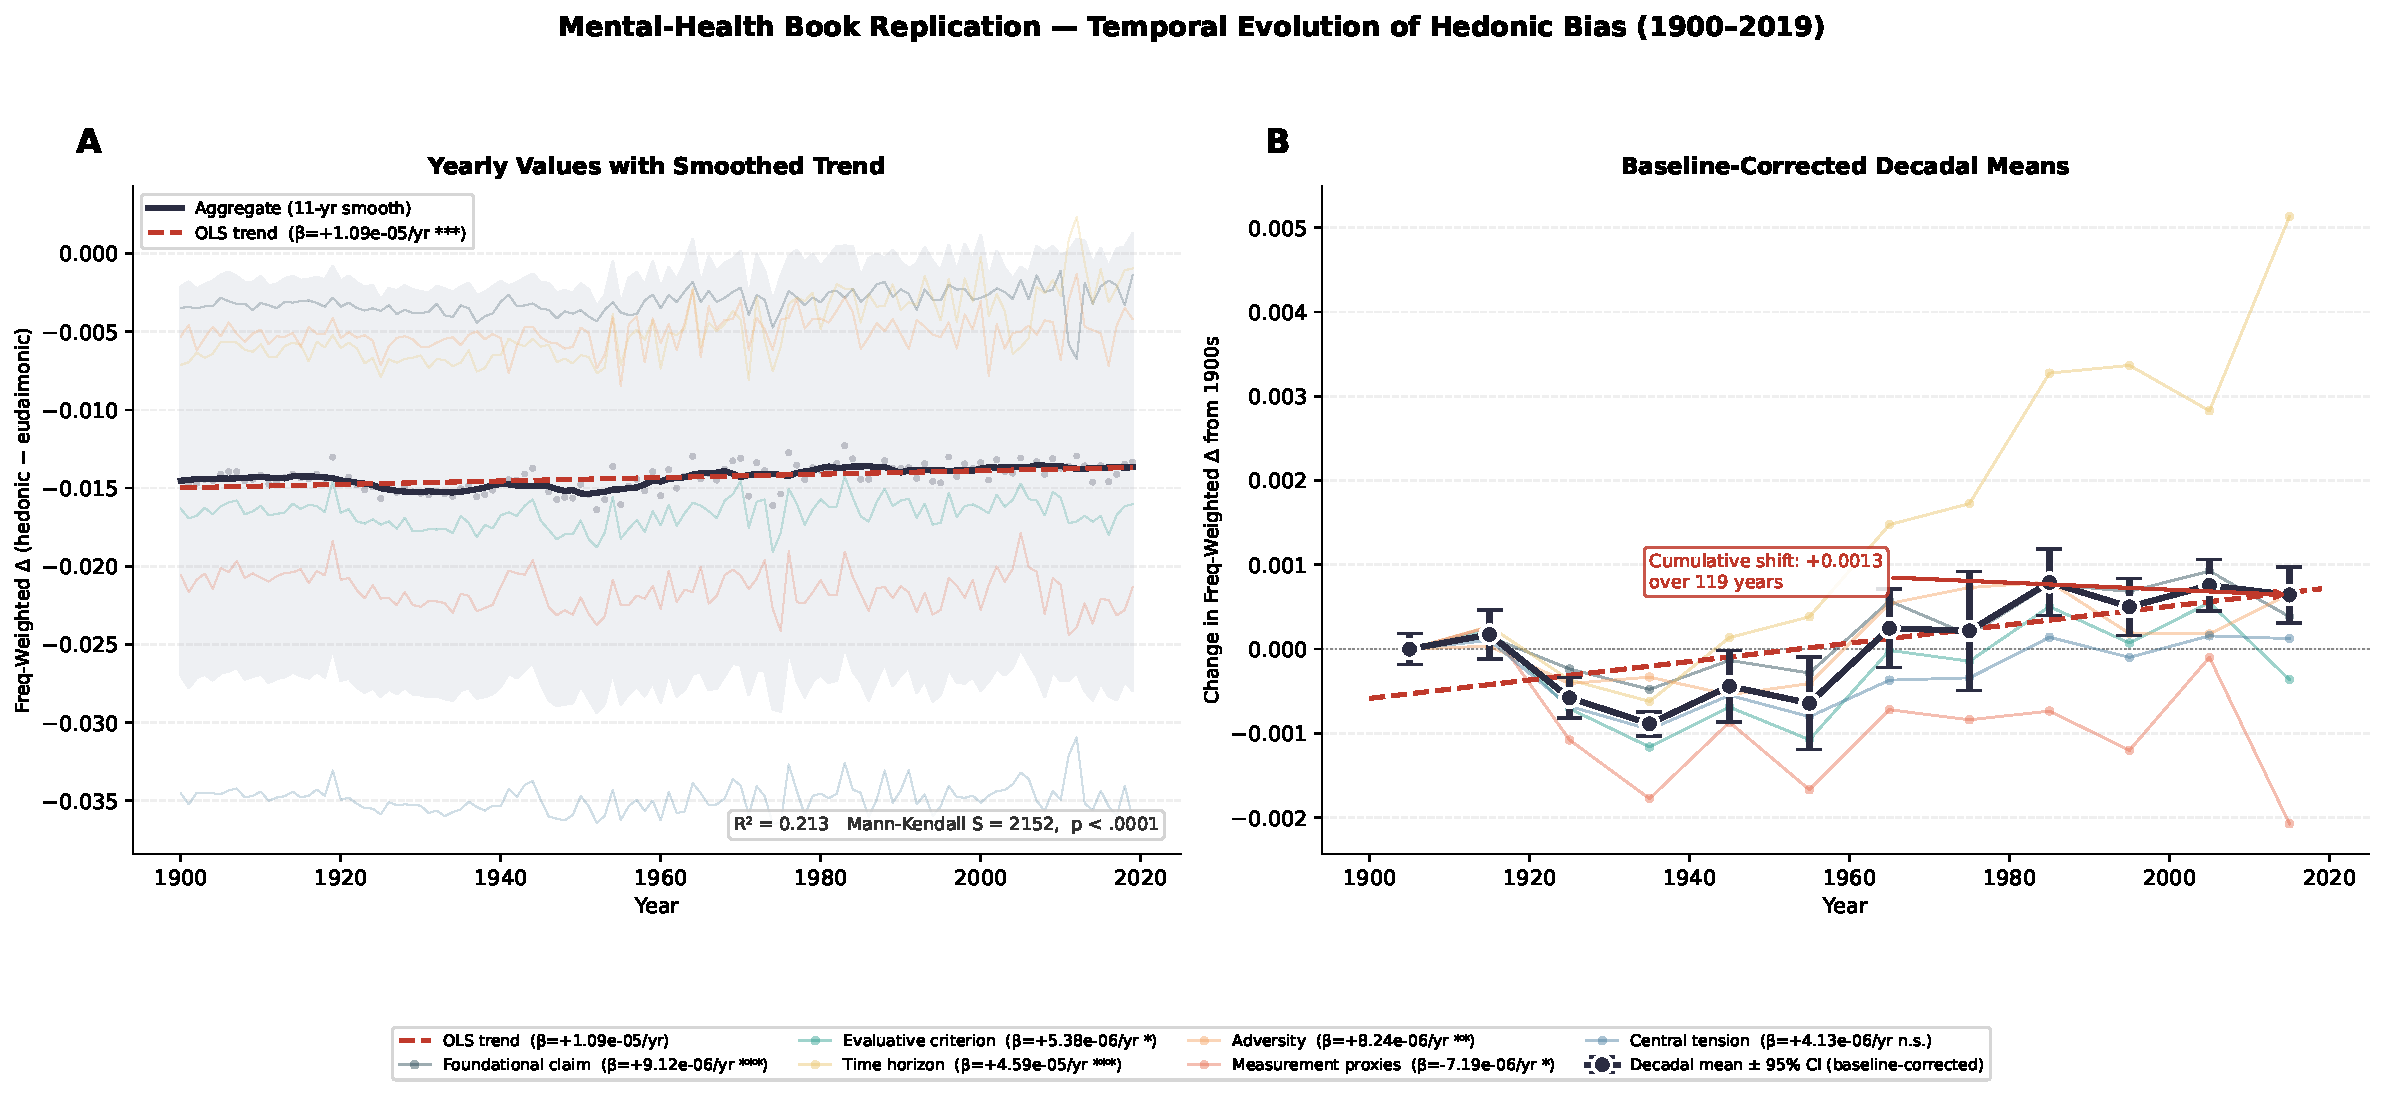
\includegraphics[width=\textwidth]{ngram_h2_combined.pdf}
    \label{fig:s_ngram_h2}
    \floatnote{(A)~Yearly frequency-weighted $\Delta$ (hedonic $-$ eudaimonic) for 9{,}285 words in 3{,}883 Internet Archive mental-health books (1900--2019). Grey dots = raw yearly values; bold curve = 11-year centred rolling average; dashed red line = OLS regression. Dimension-level series are shown as thin semi-transparent lines. (B)~Baseline-corrected decadal means with 95\% CIs, showing the cumulative shift relative to the 1900s baseline. Because each word's embedding is fixed, all temporal variation reflects shifts in relative word frequency within mental-health literature.}
\end{figure}

\subsubsection*{Interpretation}

The 120-year temporal analysis yields a striking dissociation when combined with the H1 book result.
While mental-health literature does \textit{not} exhibit a cross-sectional hedonic bias (S9), its hedonic loading has been \textit{increasing significantly} over the past century.
The aggregate trend explains a meaningful share of the variance ($R^2 = .21$) and is statistically robust across both parametric (OLS $p < 10^{-7}$) and non-parametric (Mann-Kendall $p < 10^{-6}$) tests, with bootstrap confidence intervals that exclude zero.

The lower $R^2$ compared to pre-aggregated Ngram data is expected and interpretable: whereas Ngram data averages across millions of books, smoothing out year-to-year noise, our book-level corpus comprises a finite sample of 3{,}883 volumes with uneven temporal distribution.
The resulting time series is noisier but more directly interpretable as reflecting actual variation in mental-health book content.
The Durbin--Watson statistic of $1.39$ indicates substantially less autocorrelation than the Ngram analysis (DW~$= 0.24$), meaning that the OLS $p$-values are more trustworthy for the book-level corpus.

\paragraph{Effect-size comparison with clinical H2.}
A comparison of absolute effect sizes is instructive.
The clinical H2 analysis (Section~\ref{sec:results-h2}) found a usage-weighted slope of $+4.59 \times 10^{-4}$/yr ($R^2 = .94$) over 25~years; the book-level analysis found a slope of $+1.09 \times 10^{-5}$/yr ($R^2 = .21$) over 120~years---approximately 42~times smaller in magnitude.
This ratio mirrors the H1 pattern: clinical measurement instruments exhibit a much larger hedonic bias than the broader mental-health literature.
The convergence of both cross-sectional (H1) and temporal (H2) analyses on the same conclusion---that the hedonic tilt is present in general mental-health discourse but \textit{dramatically concentrated} in clinical scales---reinforces the interpretation that psychometric design practices selectively amplify hedonic symptom content beyond what would be expected from the vocabulary of the field itself.

This temporal convergence between the book-level and clinical findings is theoretically important.
The clinical H2 analysis showed that PubMed-based scale usage has become more hedonically biased over 25~years (2000--2025); the book-level analysis extends this pattern across 120~years of mental-health literature.
The directional consistency suggests that the clinical measurement trend is not isolated to psychometric practice but mirrors a broader professional shift toward hedonic evaluative language within mental-health publishing---potentially driven by the rise of evidence-based treatment for acute symptom-focused conditions, the growth of CBT and pharmacotherapy, and the increasing influence of managed care on clinical priorities.

Combining the S9 and S10 results produces a coherent narrative: mental-health literature is not inherently hedonic-biased, but it is becoming \textit{more} hedonic over time.
Clinical measurement, which already selectively amplifies hedonic content (H1), is thus embedded within a professional trajectory that reinforces this asymmetry.
The H1 bias is a measurement-specific phenomenon; the H2 trend is a cultural and professional one, and the two compound each other.

\end{document}
